\section{Detector Infrastructure}
\label{sec:fdsp-tc-infr}


The  \dword{jpo} will provide the infrastructure needed to install the \dword{spmod}. The major items, described below, include the \dfirst{dss}, the electronics mezzanine on the cryostat roof (including racks), cable trays, an underground cleanroom with appropriate installation equipment, piping inside the cryostat, and \coldbox{}es with associated cryogenics supply. 

Other items, not described here but also in the \dword{jpo} scope, include a small machine shop, scissor lifts, rigging equipment, hand tools, diagnostic equipment (including oscilloscopes, network analyzers, and leak detectors), local storage with some critical supplies, and \dfirst{ppe}.  

%%%%%%%%%%%%%%%%%%%%%%%%%%%%
%\subsection{Detector Support System}
\subsection{Detector Support System}
\label{sec:fdsp-tc-infr-dss}

% Figure~\ref{fig:shuttle}
% \cite{bib:docdb8255}

The \dword{dss} provides the structural support for the detector inside the cryostat.  
It also provides the necessary infrastructure inside the cryostat to move the detector elements into place during assembly. 
The \dword{dss} is a new design, quite different from the \dword{pdsp} \dword{dss}. The detector elements supported by the \dword{dss} include the \dwords{ewfc}, the \dword{apa}s, and the \dwords{cpa} with top and bottom \dword{fc} panels. 
The nominal load of the detector elements both dry (in air) and wet (in \dword{lar})\footnote{The ``wet'' load takes into account the buoyancy of the liquid argon. As G10 is almost neutral buoyant the difference is substantial for some sub-systems.} are shown in Table~\ref{tab:installation-DSS-load}. 
The weights listed are the current design weights.  
The \dword{dss}, however, is designed to accommodate significant design changes --- even if the detector weight were to double the \dword{dss} still meets the design code requirements.  
The \fdth{}s can be adjusted to compensate for deflections due to load.
\begin{dunetable}
[DSS Loads]
{l|c|cc|cc}
{tab:installation-DSS-load}
{The expected dry and wet static loads for the DSS.}
%\multicolumn{2}{c}{} &  \multicolumn{4}{|c}{Dry Weight}\\ \toprowrule
& &  \multicolumn{4}{|c}%{Dry Weight}
{Weight before fill (Dry)}\\ \toprowrule
& & \multicolumn{2}{c|}{Unit Weight} & \multicolumn{2}{c|}{Total Weight}  \\ \colhline

Detector Component &\# Units& (kg)&(lbs) & (kg) &(lbs)\\ \colhline
\dword{dss} & 1 &NA&NA& 12318  & 27100 \\ 
\colhline
\dword{apa} (Installed \dword{apa} pair, no cables)& 75&1184 &2604 &88768  &195290\\ 
\colhline
\dword{cpa} & 100& 233 & 513 & 23331 & 51327 \\ 
\colhline
Top or Bottom \dword{fc} module (FC TB)& 400&149 & 328	 & 59679 & 131294\\ 
\colhline
\dword{tpc} Electronics and Cables &3000& 4.9 & 10.8 & 14700 & 32400\\
\colhline
\dword{ewfc}  & 8	&904 &	1989  & 7234 & 15914\\ 
\colhline
{\bf Total} &  & & & 206,000 &	454,000\\ 
\colhline
\toprowrule

\rowtitlestyle & &  \multicolumn{4}{c}{Weight after fill (Wet)}\\
\toprowrule
\dword{dss} (not in liquid) & 1 & NA & NA & 12318 & 27100 \\ 
\colhline
\dword{apa} (Installed \dword{apa} pair/No cables)&75&850 &1874 & 64000 &140000\\ 
\colhline
\dword{cpa} & 100& 45 & 99 & 4520 & 9943 \\ 
\colhline
Top or Bottom \dword{fc} module (FC TB)& 400 & 68 & 150	& 27359 & 60191 \\ 
\colhline
\dword{tpc} Electronics and Cables & 3000 &2.9 &6.4 & 8700& 19200 \\
\colhline
\dword{ewfc}  & 8 & 283& 	622& 2263 & 4978\\  
\colhline
{\bf Total} &  & & &110,000	 &242,000 \\ 
\colhline
\end{dunetable}


The \dword{dss} shown in Figure~\ref{fig:DSS} consists of five rows of I-beams inside the detector that support the five rows of \dword{apa}s and \dword{cpa}s. 
The I-beams themselves are supported from the cryostat outer steel structure through a series of vertical supports or mechanical \fdth{}s, also shown in Figure~\ref{fig:DSS}. 
The \dword{dss} constrains the location of the detector inside the cryostat and also accommodates the detector elements' movement and contraction during cooling. The layout of the \dword{dss} sets, in turn, the overall layout of the detector module since the module's elements become a unified mechanical structure only after they are mounted to the \dword{dss} and internally connected.

During installation the detector components are moved along the I-beams using both simple and motorized trolleys. 
The end of the \dword{dss} nearest the \dword{tco} is also designed as a switchyard. An additional set of north-south beams allow a short section of the I-beam rail to be shifted between the five rows of \dword{dss} beams that correspond to the five alternating rows of detector elements  (\dword{apa}-\dword{cpa}-\dword{apa}-\dword{cpa}-\dword{apa}).  
With this the \SI{12}{m} tall detector elements can enter the cryostat on an I-beam through the \dword{tco}, be loaded on the short switchyard beam, moved to the required row of \dword{dss} and then be pushed into position. 
\fixme{add reference to TC vol Ch 7 fig 7.6}

\begin{dunefigure}[\threed model of the DSS] {fig:DSS}
  {\threed model of the \dword{dss} showing the entire
  structure on the left along with one \dword{apa} row and one
  \dword{cpa}-\dword{fc} row at each end. The right panel is a zoomed image
  showing the connections between the vertical supports and the
  horizontal I-beams.}
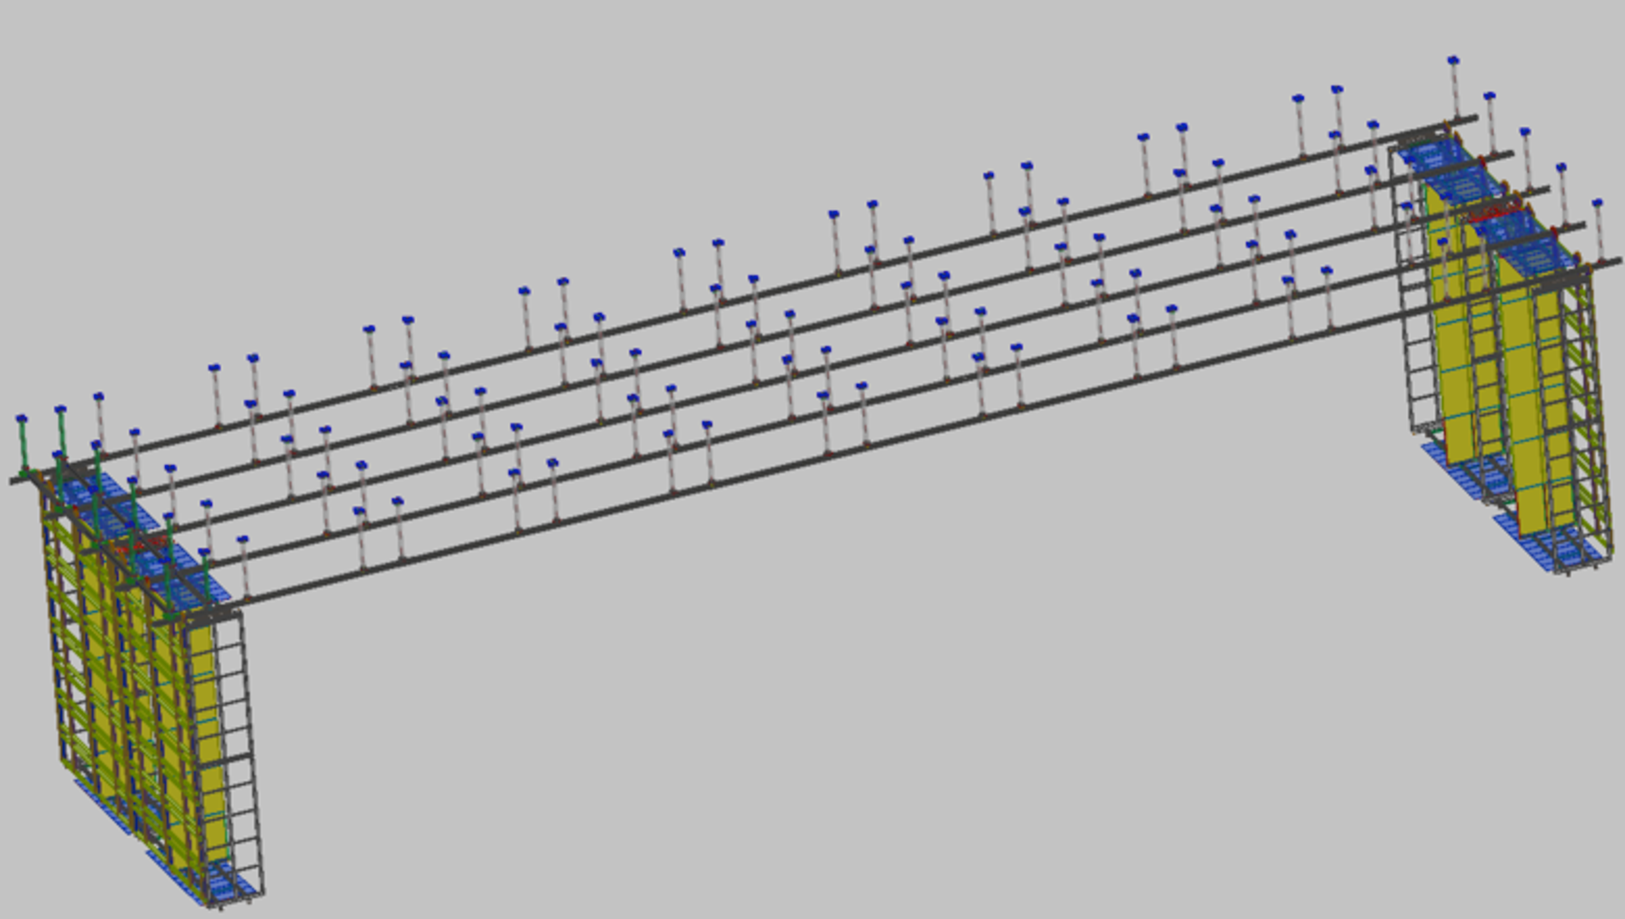
\includegraphics[width=.49\textwidth]{DSS-1.pdf}
 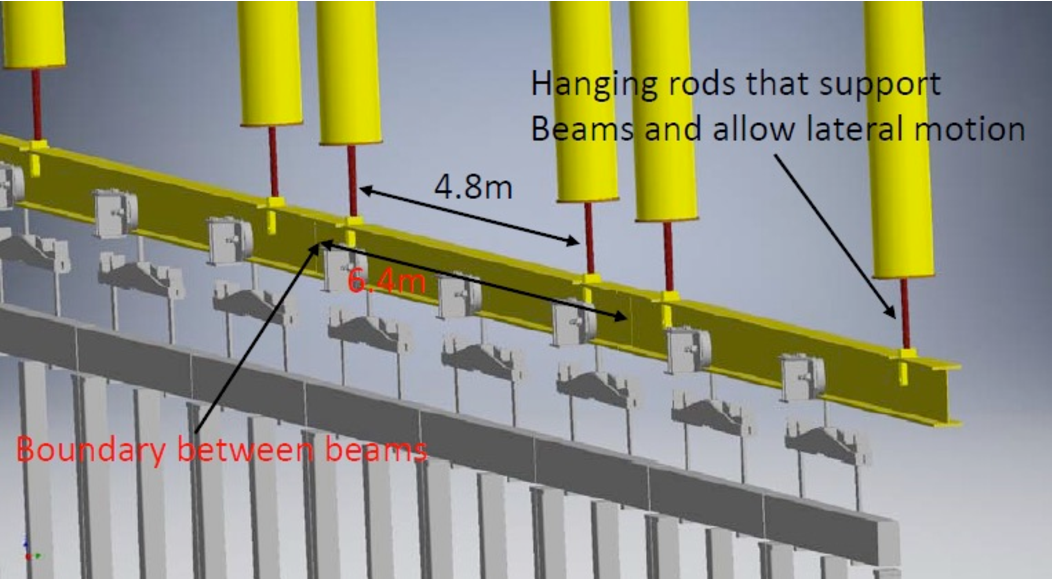
\includegraphics[width=.49\textwidth]{DSS-2.pdf}
\end{dunefigure}




The \dword{dss} is designed to meet the following  requirements:
\begin{itemize}
\item support the weight of the detector;
\item accommodate cryostat roof movement during filling, testing, and operation;
\item accommodate variation in \fdth locations and
  variation in the flange angles due to installation tolerances and
  loading on the warm structure;
\item accommodate shrinkage of the detector and \dword{dss} from ambient
  temperature to \dword{lar} temperature;
\item define the positions of the detector components relative to each other; 
\item provide electrical connection to the cryostat ground and remain electrically isolated from the detector;
\item allow support penetrations to be purged with gaseous argon to prevent contaminants from diffusing back into the liquid; 
\item ensure that the instrumentation cabling does not interfere with the \dword{dss};
\item consist entirely of components that can  
be installed through the \dword{tco};
\item meet AISC-360 codes; 
\item meet seismic requirements one mile underground at \dword{surf};
\item consist entirely of materials compatible %for 
with operation in ultrapure \dword{lar};
\item ensure that the \dword{dss} beams either sit completely submerged in \dword{lar} or sit completely in gas while leaving a \SI{4}-\SI{5}{\%} ullage at the top of the cryostat;  
%\item Centerline of the \dword{apa} near the cryostat wall shall be \SI{400}{mm} from the membrane flat surface;
\item maintain the centerline of the \dword{apa} near the cryostat at \SI{400}{mm} from the membrane flat surface;
\item ensure that the supports do not interfere with the cryostat I-beam structures;
\item ensure that the detector's lower \dword{gp} lies over the cryogenic piping; and
%and that the tops of the \dword{dss} beams are either fully submerged in \dword{lar} or fully in gas while leaving a \SI{4}-\SI{5}{\%} ullage at the top of the cryostat; 
\item include the infrastructure necessary to move the \dword{apa} and \dword{cpa}-\dword{fc} assemblies from outside the cryostat through the \dword{tco} to the correct position.
\end{itemize}

Each row of the \dword{dss} consists of a series of ten  \SI{6.4}{m} long
W10$\times$26 stainless steel I-beam sections, for a total of \num{50} I-beam segments for the five rows. The length of the beam segments was chosen to be a multiple of the \SI{1.6}{m} pitch of the major cryostat beams, which allows the regular placement of the support \fdth across the cryostat roof. With a W10$\times$26 I-beam and \SI{6.4}{m} between the supports,  the beam deflections due to the loads can be kept below \SI{5}{mm}. 
Each I-beam is suspended on both ends by the mechanical \fdth{}s that penetrate the cryostat roof. 
During \cooldown  each I-beam shrinks while the mechanical supports outside the cryostat remain fixed,  causing gaps to form between \dword{apa}s that are adjacent but supported on separate beams.
\dword{apa}s that are supported on the same beam will not have gaps develop because both the beam and \dword{apa} frames are stainless steel and will shrink together.
The gap between two adjacent \dword{dss} beams after \cooldown will be \SI{17}{mm}; this is considered acceptable. 
Increasing the the beam length beyond \SI{6.4}{m} was not considered because the deformation of the I-beam under load would increase, as would the gap between \dword{apa}s on adjacent beams and the difficulty of installing the beams. 



\begin{dunefigure}[DSS vertical support \fdth]{fig:DSS-Support}
  { Drawing of the \dword{dss} vertical support \fdth. The detector load is carried by the \SI{25}{mm} inner support rod. The outer lateral support tube prevents swinging during installation.  The \fdth mounts to the cryostat crossing tube, which is an integral part of the cryostat. 
  
  Note: A few of the \dword{dss} vertical support \fdth have a short vacuum chamber with side ports inserted between the \dword{dss} support flange and the cryostat crossing tube. These chambers are used to bring the \dword{cisc} cables out of the cryostat and are shown in the \dword{cisc} section in Figure \ref{fig:CISC-feedthru}.}
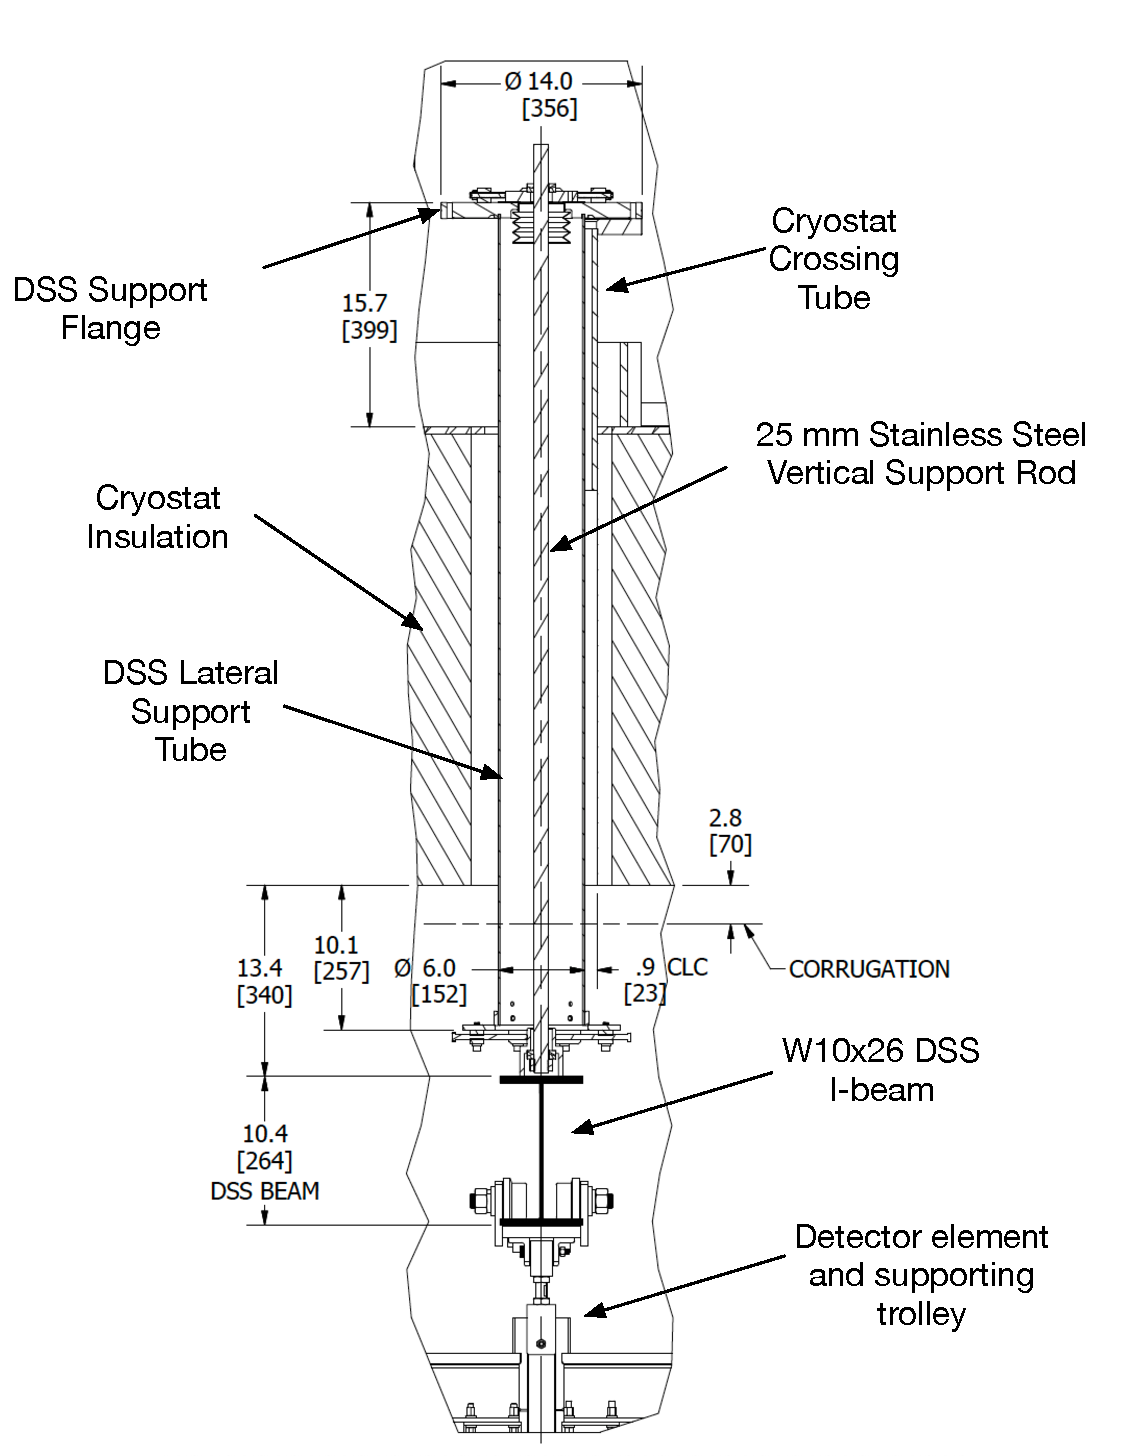
\includegraphics[width=.85\textwidth]{graphics/DSS-Support.pdf}
\end{dunefigure}


The \dword{dss} I-beams are supported on both ends from a vertical support \fdth shown in Figure~\ref{fig:DSS-Support}. A \SI{25}{mm} solid stainless steel rod, which is threaded at both ends, runs down the center of the \fdth and carries the detector load. The support rod connects on the bottom end to a clevis which is then pinned to the \dword{dss} beams shown in Figure \ref{fig:DSS-lateral-support}. At the top the rod bolts to an X-Y table sitting on the top Conflat flange that allows a lateral adjustment of $\pm$\SI{2.5}{cm} (\SI{1}{in}). A swivel washer is used in the bolted connection to the X-Y table to allow the support rod to swing freely. The bolted connection also allows the \dword{dss} I-beams to be adjusted vertically. The vacuum seal is established at the top with a bellows between the rod and the top flange. The top flange of the \dword{dss} support \fdth is a Conflat flange that connects to the cryostat crossing tube's mating flange. The crossing  tube is welded to the cryostat roof and the top flange is mechanically supported from the cryostat's  \SI{1.1}{m} tall support I-beams. The cryostat crossing tubes are shown in Figure~\ref{fig:crossingtube}.

During installation the detector components will be pushed along the \dword{dss} I-beams, placing a lateral load on the \dword{dss}. % support structure. 
A \SI{15.2}{cm} (\SI{6}{in}) \dword{od}  tube is welded to the top flange of the \dword{dss} \fdth{}. 
This lateral support tube  extends through the cryostat insulation and has a clamping collar at the bottom that is used to fix the I-beam support clevises in position during installation. 
The bottom of the lateral support tube is seen in Figure~\ref{fig:DSS-lateral-support}. 
The long bolts press on the flat sides of the clevis to fix the support rod's location. 
There is a nominal \SI{10}{mm} gap between the \dword{od} of the support tube and the \dword{id} of the clearance tube in the cryostat. 
The clevis can be positioned anywhere inside the \SI{15.2}{cm} tube.




\begin{dunefigure}[DSS support for lateral loads ]{fig:DSS-lateral-support}
  {Left panel shows how the central support rod is locked in position during detector installation. The outer  \SI{15.2}{cm} (\SI{6}{in}) tube is used to fix the support clevis in position. The right panel shows the system as it is connected to the I-Beam.}
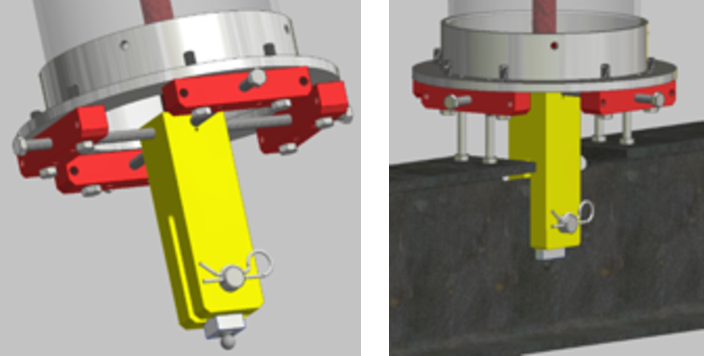
\includegraphics[width=.75\textwidth]{graphics/dss-lateral-support.pdf}
\end{dunefigure}

After the detector has been installed all restraints on the clevis are released to allow motion as the detector contracts during \cooldown.  The two support rods that support each \dword{dss} beam will contract and move toward each other by \SI{13.1}{mm} along the axis of the detector.  
The drift distance will shrink by \SI{7.4}{mm}  caused by the contraction of the field cage.  The detector is symmetric in the drift direction around the center \dword{apa}.  The drifts on either side of the center \dword{apa} will  shrink toward the center while the center \dword{apa} remains unmoved.  This results in the \dword{cpa}s moving \SI{7.4}{mm}  toward the center and the outer \dword{apa}s moving \SI{14.8}{mm}  (2$\times$\SI{7.4}{mm}) toward the center.  The hanging rod is designed to have a range of motion of \SI{15}{mm}  in the drift direction to accommodate this shrinkage.




Detector components are installed using a shuttle beam system as
illustrated in Figure~\ref{fig:shuttle}.  
The last two columns of \fdth{}s (western-most) support temporary beams that run
north-south, perpendicular to the main \dword{dss} beams.  
A shuttle beam has trolleys mounted to it and traverses 
north-south until it aligns with the required row of \dword{dss} beams.  
The last \dword{apa} or \dword{cpa} in a row is supported by the shuttle beam, which is bolted directly to the \fdth{}s once it is in place.  
As the last \dword{cpa} or \dword{apa} in each row is installed, the north-south beams are removed. This system will be thoroughly tested as part of the Ash River testing program described in \ref{sec:fdsp-tc-inst-qaqc}.

\begin{dunefigure}[\threed models of the shuttle beam end of the DSS]{fig:shuttle}
  {\threed models of the shuttle beam end of the \dword{dss}. The figures show how an \dword{apa}
is translated into position using the north-south beams until it lines up with the correct
row of I-beams.}
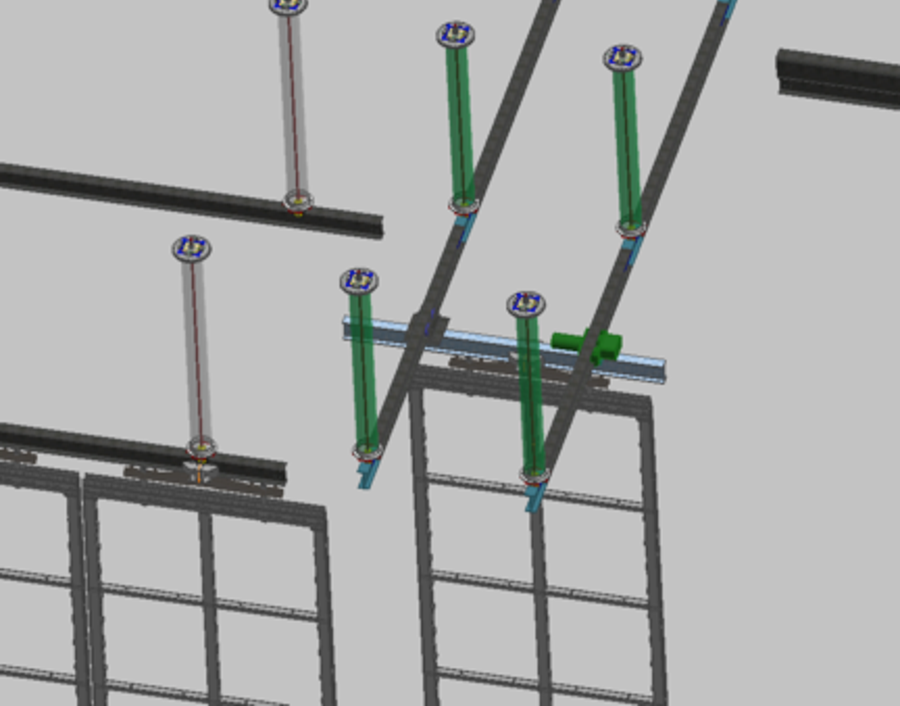
\includegraphics[width=.49\textwidth]{/Shuttle-1.pdf}
 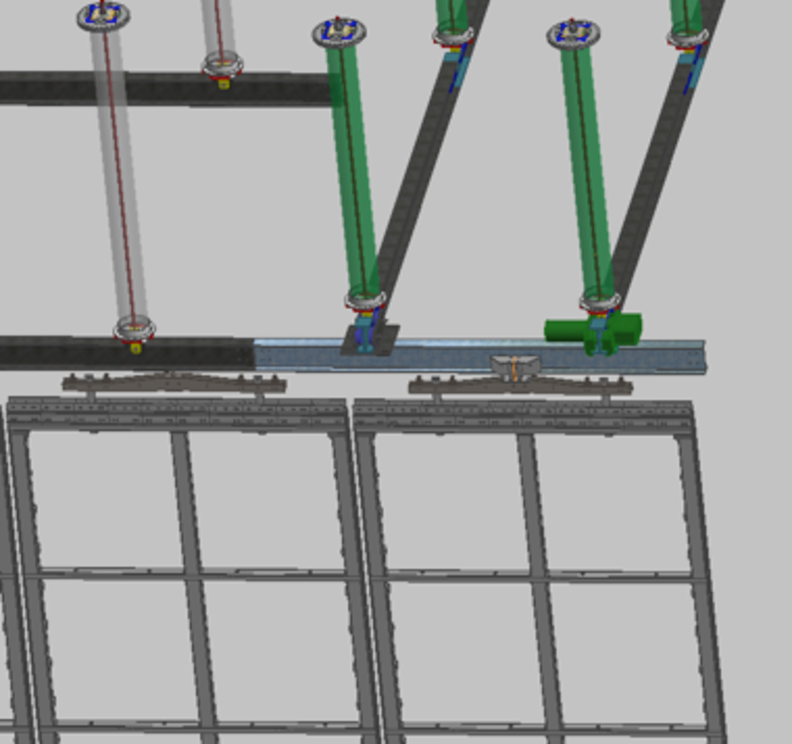
\includegraphics[width=.42\textwidth]{shuttle-2.pdf}
\end{dunefigure}

The shuttle beam and each detector component are moved using a motorized trolley as seen in Figure \ref{fig:DSS-trolley}.  A commercially available motorized trolley will be modified as needed for the installation. A mechanical stop will prevent the trolley from passing the end of the shuttle beam unless the beam is aligned with a corresponding \dword{dss} beam. A detailed engineering design report for the \dword{dss} is available \cite{bib:docdb6260} and the preliminary design review is complete.

\begin{dunefigure}[Prototype of the motorized DSS trolley ]{fig:DSS-trolley}
  {Prototype of the motorized \dword{dss} trolley that will push the \dword{apa} and \dword{cpa} along the I-beams and through the switchyard.}
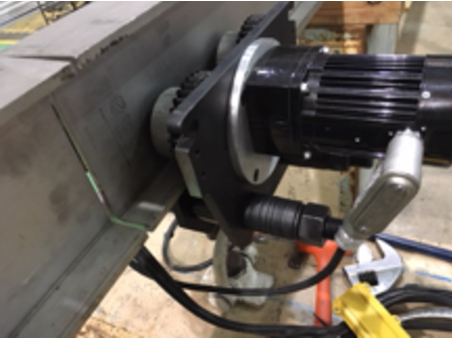
\includegraphics[width=.49\textwidth]{graphics/DSS-trolley.pdf}
\end{dunefigure}



A mock-up of the shuttle system will be constructed to test the mechanical interlock and drive systems for the shuttle beam for each \dword{detmodule}.  
Tests will be conducted to evaluate the level of misalignment between beams that can be tolerated and the amount of positional control that can be achieved with the motorized trolley. 
We plan to construct a full scale prototype of a section of the  switchyard and perform tests at floor level. 
Later, the test program will be expanded at Ash River, where a full-scale installation test will be performed; see Section~\ref{sec:fdsp-tc-inst-qaqc}.


%%%%%%%%%%%%%%%%%%%%%%%%%%%%
\subsection{Cryostat Roof Infrastructure}
\label{sec:fdsp-tc-infr-cryo-roof}

\begin{dunefigure}[Mezzanine and electronics racks]{fig:mezzanine}
  {The electronics racks sit on the \dword{dune} electronics mezzanine. The top image is a view from above the detector looking at the racks from the side. In this view the cavern and cryogenics mezzanine are hidden. The bottom view is from the end of the cryostat looking over the roof. The access stairs to the mezzanine are shown.}
 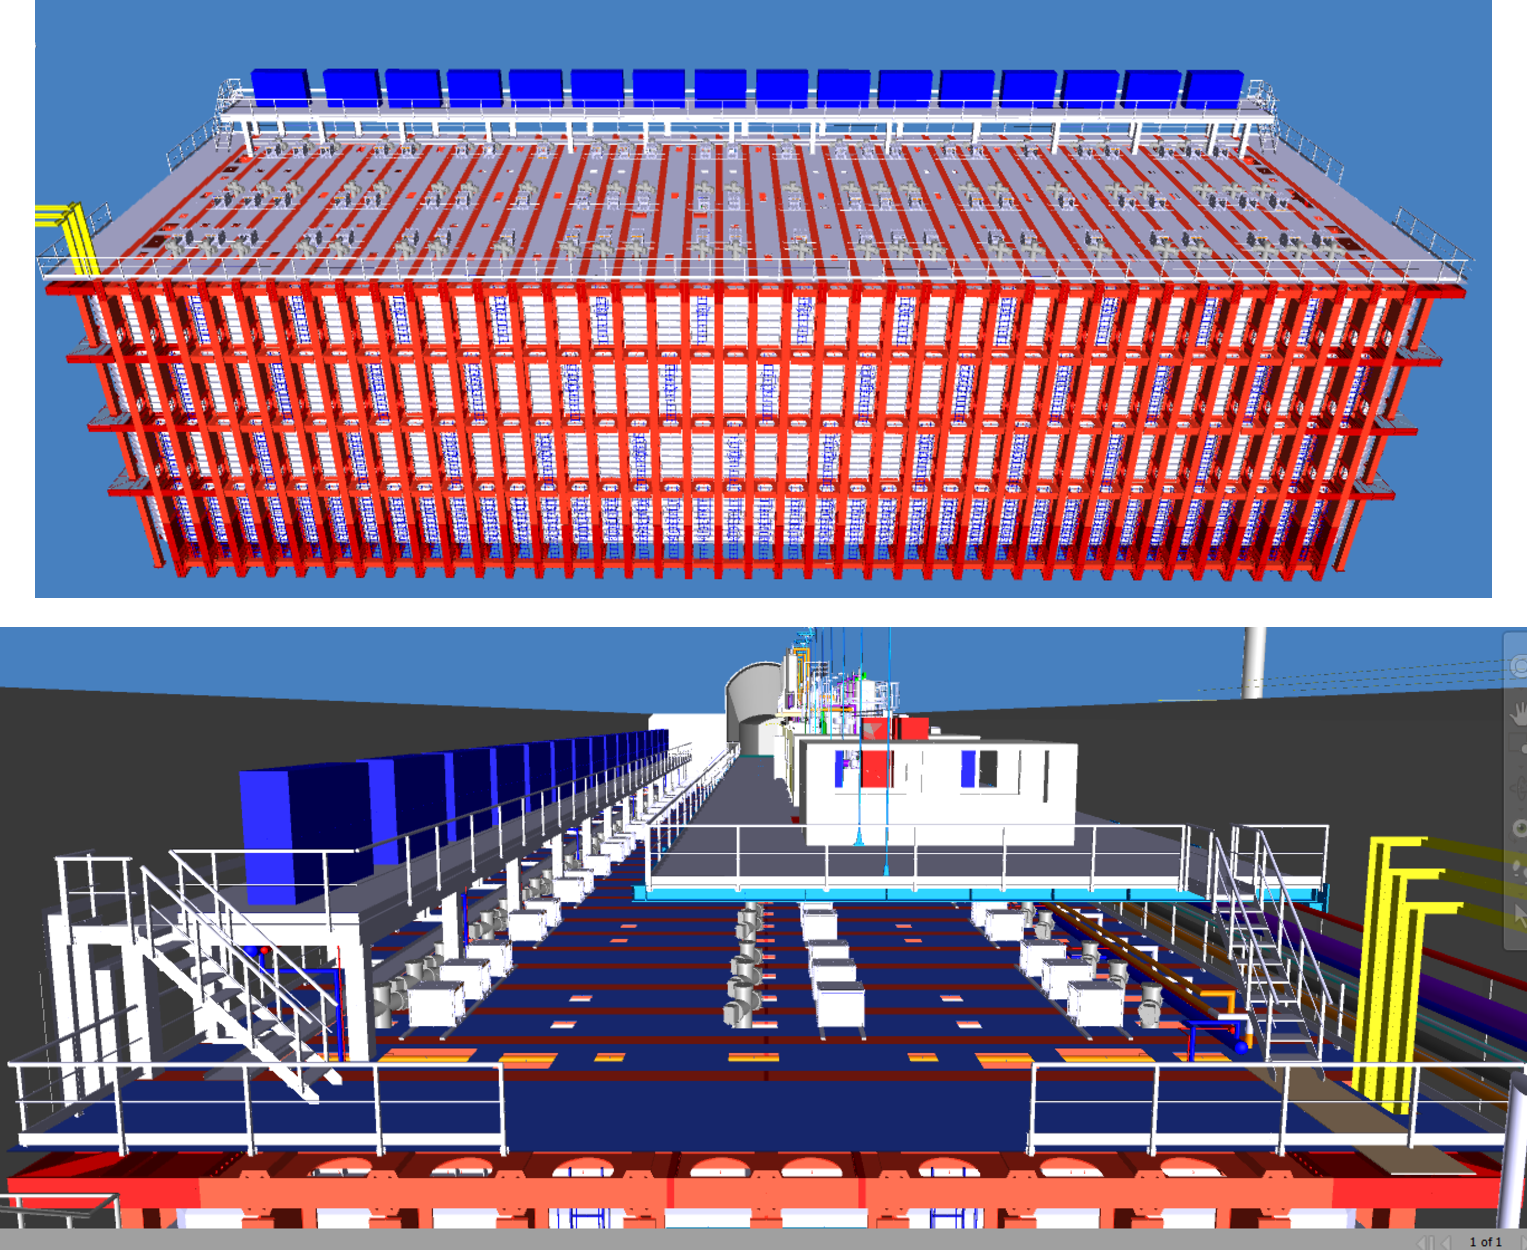
\includegraphics[width=\textwidth]{mezzanine.pdf}
\end{dunefigure}

\begin{dunefigure}[Electronics rack contents]{fig:rack-build1}
  {The nominal contents of the electronics racks on the mezzanine is shown. Each rack is configured to consume less than 3.5 \si{kW}. \fixme{Weiner is mis-spelled in the table should be Wiener. Need update from Terri}
  }
 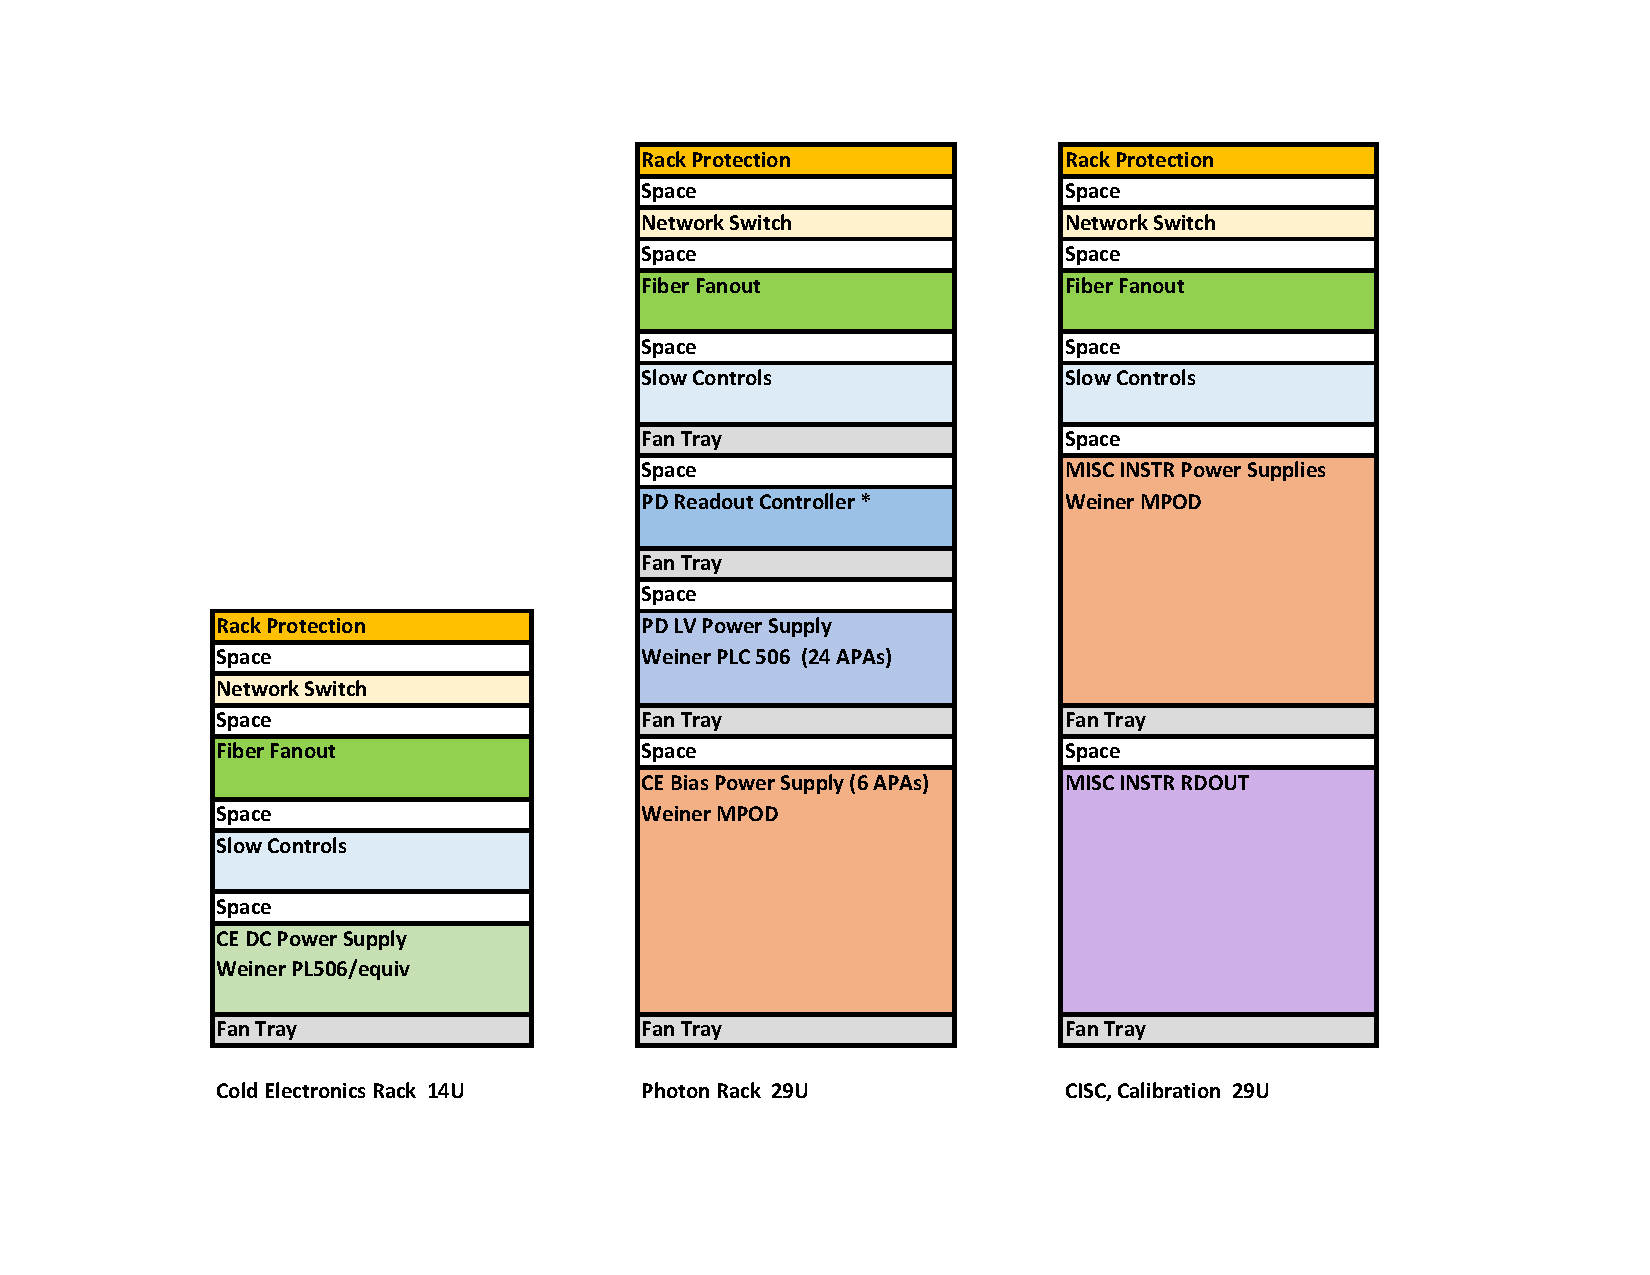
\includegraphics[width=.8\textwidth]{rack-build1} 
\end{dunefigure}

The top image in Figure~\ref{fig:mezzanine} shows the \dword{dune} electronics mezzanine with the 42U tall racks placed on top. 
During the initial design steps, it became clear that the constraints placed on the rack location by the many \dword{dss} support \fdth{}s, the electronics \fdth, and the I-beams themselves make distributing the racks on the roof very challenging. 
By constructing a fixed mezzanine for the electronics above the cryostat at the same height as the cryogenic mezzanine, the electronics \fdth{}s are kept clear. 
This configuration also makes working on the electronics much easier because there are no local obstacles and all the racks are in one place.

Since the electronics modules in the  racks are connected to the detector readout electronics, they are by definition at detector ground. The mezzanine must therefore also be connected to detector ground, which is accomplished by bolting the mezzanine to the cryostat I-beams. 
 \fixme{Need input from Terri related to the exact text of the mezzanine ground. (Anne - still needed? 10/17}
 
Figure \ref{fig:mezzanine} (top) shows 16 groups of five racks each
on the mezzanine for a total of 80 racks. 
The electronics inside the detector racks will be air-cooled and the heat exhausted into the cavern air. The HVAC system for the detector cavern has a \SI{400}{kW} capacity, which is sufficient for the first \dword{detmodule}.  Note that as the majority of the heat is generated by the \dword{ce} \fixme{should this be TPC electronics?} and \dword{pd} electronics located near the cryostat \fdth{}s distributed across the cryostat roof, a water-cooling scheme would be difficult to engineer.
 \dword{cf} will provide sufficient chilled water capacity at the entrance to the north cavern to accommodate the maximum heat load for two \dwords{detmodule}. When detector \#3 is selected and the heat loads are known, the added cooling for this module will be designed.



Of the 80 racks, \dword{ce} \dword{lv} power requires \num{25}, and another \num{25} will be made available collectively for  \dword{apa} wire bias voltage, \dword{pd} power, and miscellaneous additional \dword{ce}, \fixme{tpc elec?} \dword{pds}, and  \dword{apa} electronics modules. 
The remaining 30 will be available for slow control, calibration, and other electrical equipment. 
Small 12U-high mini-racks will  be placed near the electronics \fdth{}s for the \dword{pd} readout electronics and optical patch panels. If this is not enough, additional racks can be placed on the cryostat roof. The present rack configuration for this layout is shown in Figure~\ref{fig:rack-build1}. 
The electronics modules inside the racks are distributed to keep the AC power requirement for each rack below \SI{3.5}{kW}. 
The racks are 42U high, which provides significant extra rack space~\cite{bib:docdb4499}.  


The 12U-high mini-racks near the \fdth flanges will be relatively empty because the \dword{pd} readout should need only approximately 2U in height while the \dword{ce} patch panel needs less than 1U. The mini-racks are shown in the lower panel of Figure~\ref{fig:mezzanine}; 
they are the gray rectangles near the electronics crosses.

The north-south cable trays (transverse to the beam) that run from the electronics mezzanine to the electronics \fdth are routed under the floor of the cryostat roof (shown in gray in Figure~\ref{fig:mezzanine}) next to the 
I-beams. 
This keeps the roof reasonably clear, allowing equipment to be transported across it. 
The gap between the web of the I-beams is \SI{1.2}{m} so 
a \SIrange{200}{300}{mm} wide cable tray installed along the beams 
leaves enough space for people to work on the electronics crates while standing directly on the cryostat's outer steel skin (Figure~\ref{fig:install-elect-cross}). 
The cable trays between the \dword{cuc} and the electronics mezzanine will run along the west end of the cryostat under the floor of the cryostat roof. 
We estimate that only half of the \SI{1.6}{m} space is needed, so the cable tray quantity could in principal be doubled, if necessary. 

The flooring material for the \dword{spmod}
will be similar to the \SI{25}{mm} thick plywood used at \dword{pdsp}. 
It is important that it be easy to cut so that it can be fit around many obstacles and pipes on the roof.  \fixme{not obvious why it needs to fit around obstacles on the roof. Anne}
It must be light enough to lift up to allow access under the floor, and it must support the load of a person and a small cart. 
We will investigate fire-retardant options available in the USA and other possible materials, with input from the \dword{fnal} fire life-safety group. 

Air filters for the clean room and inside the cryostat will also be placed on the cryostat roof. The present plan is to place fan filter units near the %manholes 
access holes on the east end of the cryostat. Initial calculations indicate sufficient airflow is possible to support one air exchange per hour inside the cryostat. The air handling system has yet to be designed in detail.


\begin{dunefigure}[Cryostat crossing tube design]{fig:crossingtube}
  {Draft drawing of the cryostat crossing tubes. The hatched region is the cryostat insulation. Units are mm. Points labeled ``u'' and ``v'' are welds. }
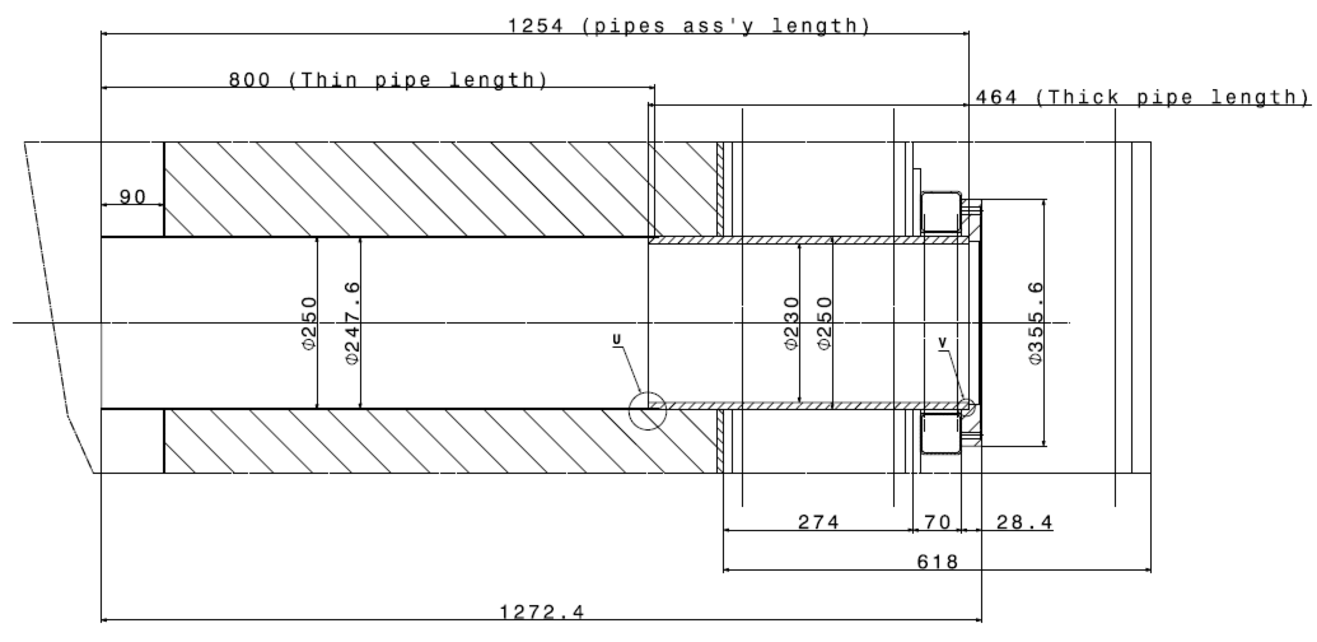
\includegraphics[width=.85\textwidth]{crossingtube}
\end{dunefigure}
 
The cryostat crossing tubes are among the most critical components of the roof infrastructure since they penetrate the cryostat roof and connect to the cold cryostat membrane. The top flange of the crossing tube supports either the electronics \fdth or the detector support \fdth and must be directly tied to the cryostat's steel I-beams for support. 
Accurate placement and true vertical installation of the crossing tubes is important to ensure proper interfacing to the cryostat membrane. 
A draft assembly drawing of the crossing tube is shown in Figure~\ref{fig:crossingtube}. 
The crossing tube consists of a \SI{464}{mm} long stainless steel pipe with a \SI{1}{cm} thick wall. 
One end of the thick-walled section is welded to a \SI{800}{mm} long \SI{250}{mm} diameter thin-walled tube which is also welded to the cryostat membrane.
A custom Conflat flange at the top end of the crossing tube connects to the \fdth. 
The thick tube section is also welded to the steel roof plates (the thin cross-hatched segments in Figure~\ref{fig:crossingtube}).  

 
Each of the 250 crossing tubes has a small side port that connects to the cryogenic gas-handling system through a network of pipes on the cryostat roof. During the initial purge \dword{gar} is withdrawn from each port and analyzed to assess progress and determine when the system is ready to be cooled down. Five \dword{gar} streams, each collecting gas from 50 crossing tubes, are connected independently to the gas analyzers. This provides some redundancy and position-dependant information on the contamination level of the gas at the top of the cryostat during the purge.
 
During filling and normal operation the collection and analysis of the gas from the crossing tubes will continue in order to monitor impurities (mainly water, oxygen and nitrogen) produced by outgassing from the cables in the \fdth{}s and the warmer metal surfaces in the ullage. These impurities can be removed from the \dword{gar} by the cryogenics system.
If the gas analyzers find no significant nitrogen contamination, the \dword{gar} from all or a subset of ports can be sent to the condenser, re-condensed, and purified along with the rest of the \dword{lar}. Simple O$_2$\ sensors monitor the return gas for traces of oxygen, which would indicate development of a leak in the room-temperature \fdth{}s.

A \SI{500}{kVA} transformer provides power to each \dword{detmodule} and the total power budget available for use by detector electronics is derated to \SI{400}{kW} at the power distribution panels.  
The \dword{ce} is the \dword{spmod}'s largest power consumer,  dissipating \SI{306}{W} per \dword{apa}.  
The \dword{lv} power supplies' controller needs about \SI{35}{W} per \dword{apa} and has an efficiency of approximately \SI{85}{\%}. 
This leads to a load of  approximately  \SI{400}{W}  per \dword{apa}, or a total load of  \SI{60}{kW} per \dword{detmodule}.  
The \dword{apa} wire-bias power supplies have a maximum load of  \SI{465}{W} per set of six \dword{apa}s, for a total budget of about   \SI{12}{kW}.   
Cooling fans and heaters near the \fdth{}s will use a nominal amount of power, so the overall power budget for the \dword{ce} and  \dword{apa}s is expected to be less than \SI{75}{kW}.


The \dword{pds} electronics is based on the \dword{mu2e} cosmic ray veto electronics, which reports a power load of approximately  \SI{6}{kW}.  \dword{dune} plans a power budget of  \SI{8}{kW} because of cable drops and  power supply inefficiencies.  

Each of the approximately 80 detector racks will have fan units, Ethernet switches, rack protection, and slow controls modules, adding a load of about \SI{500}{W} per rack, for a total of \SI{40}{kW}.

Twenty-five racks are reserved for cryogenics instrumentation with a per-rack load conservatively estimated at \SI{2}{kW}, for a total of \SI{50}{kW}. 

The \dword{detmodule} will thus use  an estimated \SI{173}{kW} of power.   These numbers provide a safety factor of about two on our power estimates relative to available power.


%%%%%%%%%%%%%%%%%%%%%%%%%%%%  anne to here 10/17
\subsection{Cryostat Internal Infrastructure}
\label{sec:fdsp-tc-infr-cryo-int}

%%%%Internal Cryogenics%%%%
\label{sec:fdsp-tc-internal-cryo}

The internal cryogenics comprises three sets of pipe distribution networks and two sets of sprayers. All pipes enter the cryostat from the top; some go all the way down to the floor, and others remain in the ceiling. On the floor are:
\begin{itemize}
\setlength\itemsep{1mm}
\setlength{\parsep}{1mm}
\setlength{\itemsep}{-5mm}
\item \textbf{\dword{gar} distribution}: a set of pipes %flowing 
for \dword{gar}. These pipes are used only prior to filling %at the beginning 
to remove air %that fills 
in the cryostat. They will all have either a longitudinal slit or calibrated holes to distribute \dword{gar} uniformly along the length of the cryostat. 
We have run \dword{cfd} simulations showing that air will be removed from the system as long as \dword{gar} is flowing in at the right speed, calculated and experimentally verified as \SI{1.2}{m/hr} (vertical meters in the cryostat).  


\item \textbf{\dword{lar} distribution}: two sets of pipes are required for flowing 
\dword{lar} over a broad  range of flow rates. These pipes are used to fill the cryostat and, during steady state operations, to return the \dword{lar} from the purification system. The pipes have calibrated holes to return the \dword{lar} uniformly throughout the length of the cryostat. This is very important %for 
to maintain uniform purity. Four pumps circulate the \dword{lar} inside the cryostat, all of which operate %. Initially, all of pumps operate at once 
initially to achieve purity. %but 
Once the target purity is achieved, only one or two pumps remain in service. %Two sets of pipes are needed to adequately distribute the \dword{lar} over this broad range of flow rates.
\end{itemize}

On the ceiling are:

\begin{itemize}
\setlength\itemsep{1mm}
\setlength{\parsep}{1mm}
\setlength{\itemsep}{-5mm}
\item \textbf{Cool down sprayers}: Two sets of cool down sprayers are distributed along the long sides of each cryostat. One set distributes \dword{lar} using liquid sprayers that generate a conical profile of small droplets of liquid. The other set of sprayers distributes \dword{gar} to move the \dword{lar} droplets inside and cool down the detector and cryostat uniformly. These sprayers are being tested in \dword{pddp}. They are a variation of those implemented in \dword{pdsp}.
\end{itemize}

Figure~\ref{fig:internal-cryo-3D} shows the current layout of the internal cryogenics. 
%The current drawing of the internal cryogenics is presented in Figure~\ref{fig:internal-cryo-drawing}. 
The \dword{gar} pipes are in red, the \dword{lar} pipes in blue.

\begin{dunefigure}[Layout of the internal cryogenics piping]{fig:internal-cryo-3D}
  {Layout of the internal cryogenics piping.}
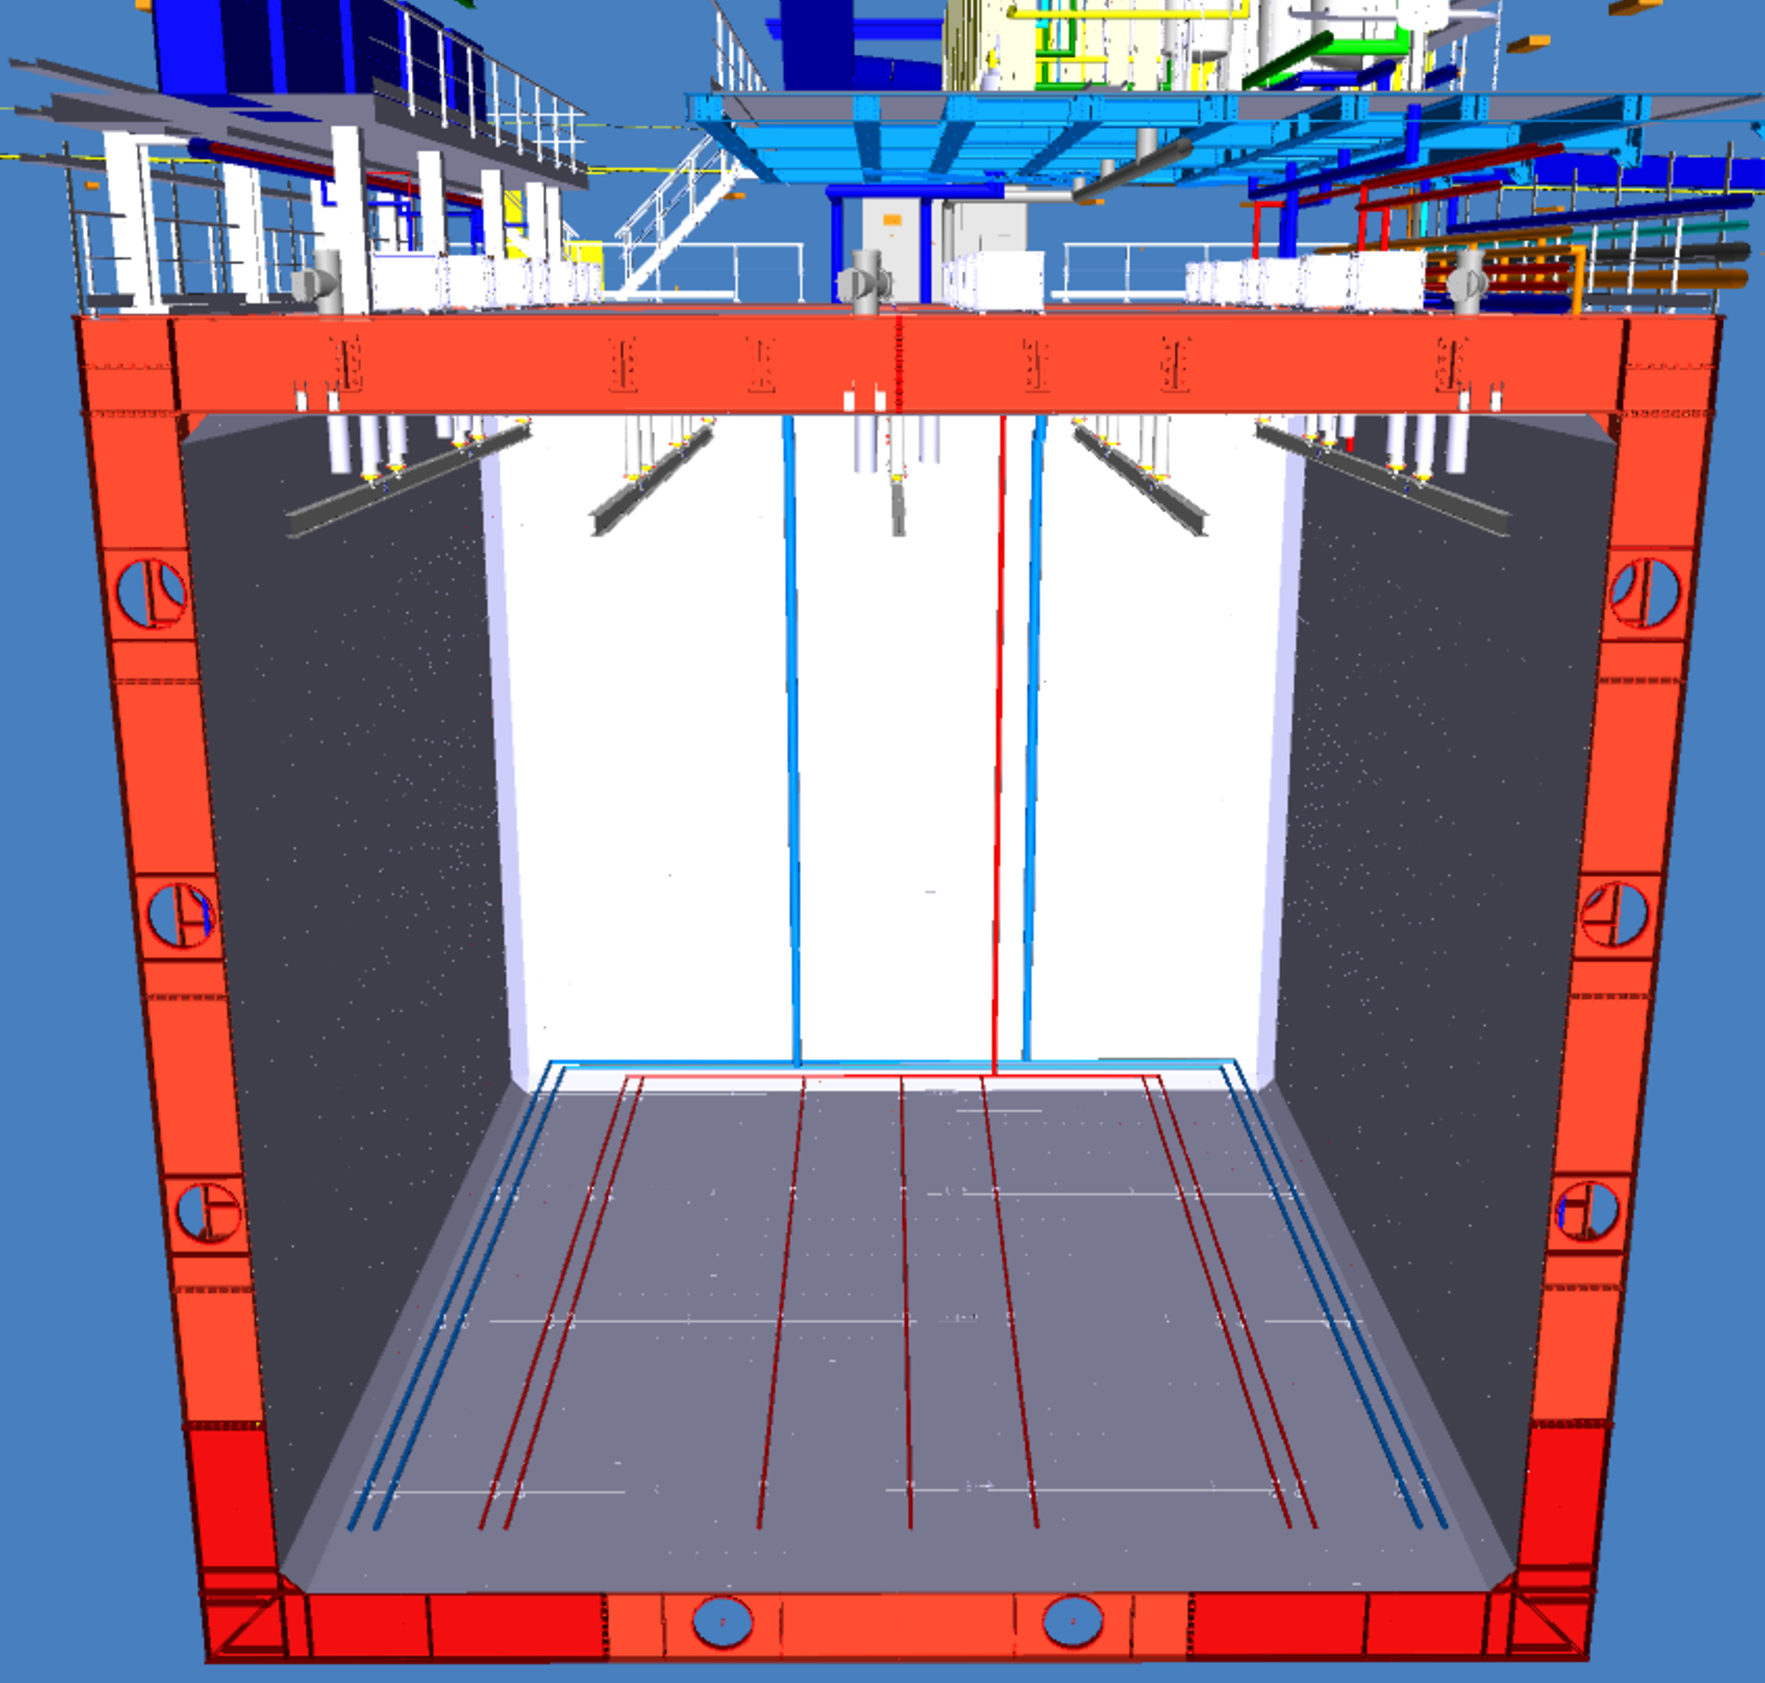
\includegraphics[width=.98\textwidth]{graphics/Internal-Piping-3D.pdf}
\end{dunefigure}

%\begin{dunefigure}[Drawing of the cryogenic %piping inside the cryostat %]{fig:internal-cryo-drawing}
%  {Drawing of the internal cryogenics.}
%\includegraphics[angle=90,width=.98\textwidth]{%graphics/Internal-pipes-HQ.pdf}
%\includegraphics[angle=90,height=.98\textheight%]{graphics/Internal-pipes-HQ.pdf}
%\end{dunefigure}
%\fixme{Please reduce size of Internal-pipes-HQ.pdf}


Other infrastructure inside the cryostat includes the cryostat false floor, the UV-filtered lighting, and the battery-operated scissor lifts. 
The floor must support the load of the scissor lift used to work on the electronic cabling on the inside of the cryostat near the ceiling and allow the scissor lift to get close enough to the \dword{apa}s to work comfortably at the top. 
The floor  must be laid out so that the panels can be removed in sections as equipment is installed. 
This is especially important for the \dword{apa}s since inadequate room exists between the bottom of the \dword{apa}s and the floor to allow removal of panels after installation. 

The cryostat lighting, using UV-filtered\footnote{Light is filtered according to the requirement SP-INST-6} \dword{led} lamps, is expected to be fairly simple. Options for the lighting will be developed during tests at the \dword{ashriver} facility.
Floor-mounted lights with task lighting will be investigated. If needed, lighting can also be mounted to the \dword{dss} and removed as the detector is installed.

We plan to use a commercially available battery-operated scissor lift with a \SI{12}{m} reach. Tests at \dword{ashriver} will verify the stability of the lift at height. If the lift is determined to be suitable, then the remaining issue to resolve is how to install and remove it from the cryostat. 
Commercially available scissor lifts are too wide to fit easily through the \dword{tco} opening where one of the large cryostat support I-beams protrudes above the TCO floor level,  so 
custom lifting equipment will be needed to insert the lifts into the cryostat from above. 
At the end of the installation process, the last lift may require dismantling before it can be removed from the cryostat.

% clear the figure buffer before starting the next section
%\clearpage

%%%%%%%%%%%%%%%%%%%%%%%%%%%%
\subsection{Cleanroom and Cleanroom Infrastructure}
\label{sec:fdsp-tc-infr-comm}

\begin{dunefigure}[Installation Cleanroom layout]{fig:install-cleanroom}
  {Two views of the installation cleanroom.  The top view shows the cleanroom in position in the north cavern. The location of the material airlock and the changing room are indicated. The lower image is a closer view showing the equipment in the cleanroom. The cryostat is shown in red.
  } 
%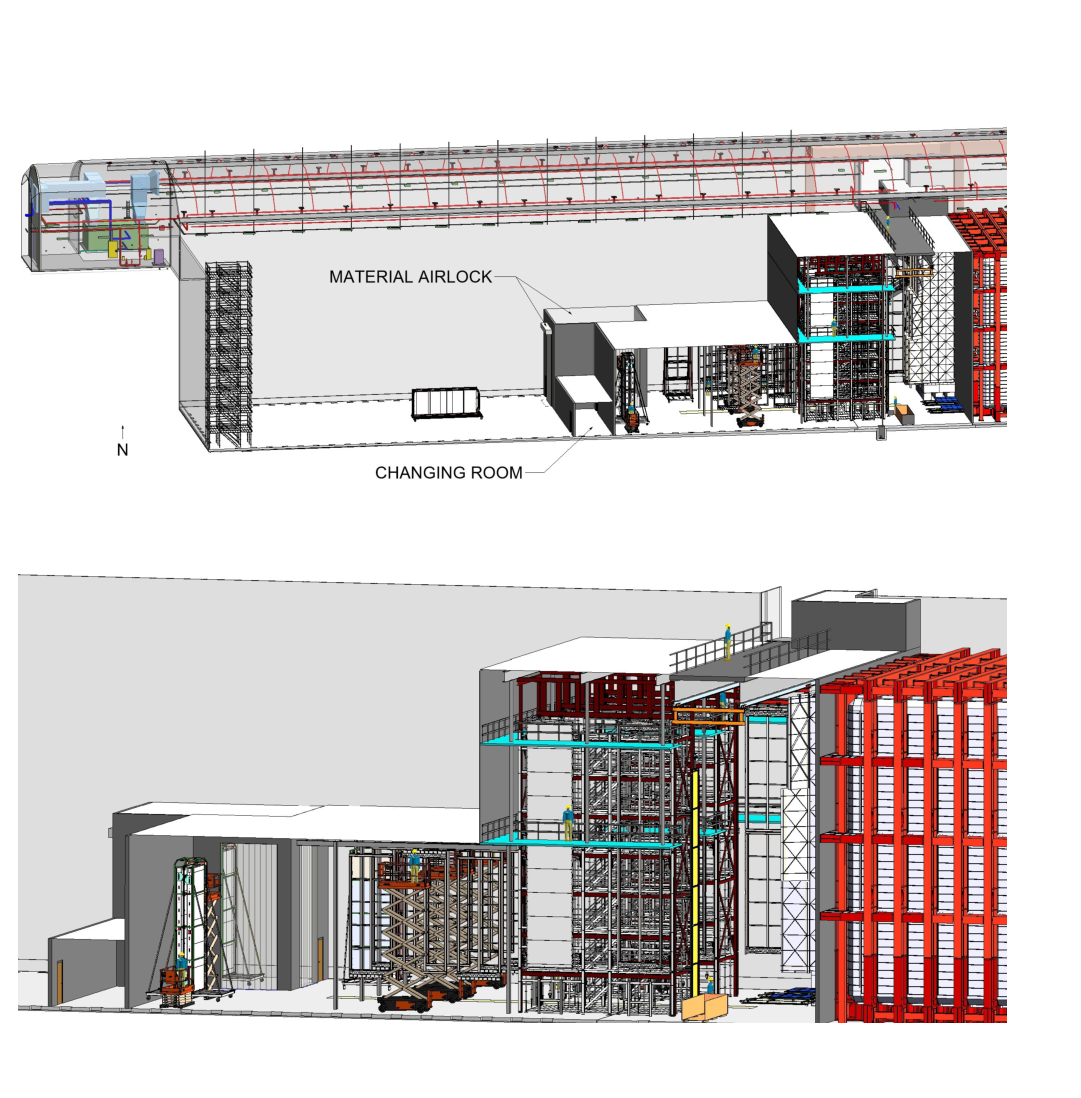
\includegraphics[width=1.0\textwidth]{graphics/install-cleanroom.pdf}
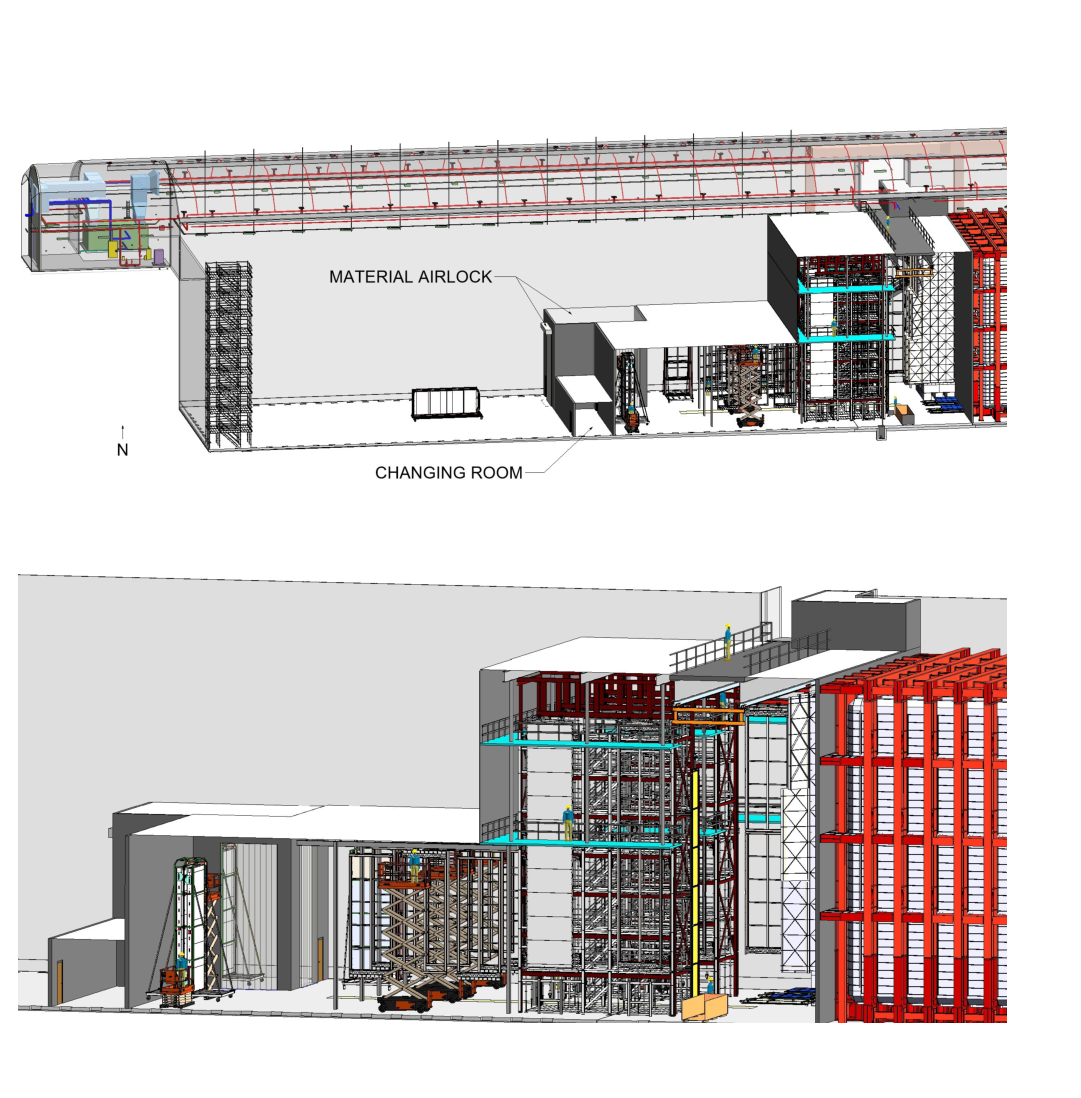
\includegraphics[width=1.0\textwidth]{graphics/install-cleanroom.pdf}
\end{dunefigure}


Since the \SI{12}{m} tall full assemblies are too large and fragile to be brought down the Ross Shaft, and the only place with enough vertical space to assemble them is in front of the cryostat itself, this is where they will be assembled. A cleanroom meeting the ISO-8 cleanroom standard is required for any work on the detector components in order to meet the \dword{dune} cleanliness requirements so a large cleanroom for the installation is planned Figure \ref{fig:install-cleanroom}.   
If the cleanroom meets the ISO-8 specification (3.5M particles per m$^3$ or 0.1M per ft$^3$) then the accumulated U/Th contamination due to dust in the detector will produce a background rate smaller than the unavoidable Ar$^{39}$ decay background.

Upon arrival in the cavern, the detector elements first pass through a materials airlock (Figure~\ref{fig:install-cleanroom}) before entering the cleanroom. This airlock has large entry doors of dimensions \SI{3}{m} wide and \SI{8}{m} tall, large enough to allow the tallest item -- an \dword{apa} transport box (\SI{2.6}{m} by \SI{6.6}{m}) -- to enter in a vertical orientation while bolted to a custom pallet and moved with electric pallet jacks. 
The airlock itself is \SI{7}{m} wide, \SI{9}{m} deep, and \SI{9}{m} tall. All materials must be brought through the material airlock and cleaned prior to entering the cleanroom proper. 
The materials airlock, cleanroom, and inside the cryostat will be outfitted with UV-filtered lights to protect the \dwords{pd}. 
Personnel must enter the cleanroom through a changing room. The changing room on the 4910 level is 13 \si{m} wide and 4 \si{m} deep where the dimensions were chosen to allow 50 people to gown up for the cleanroom within a reasonable time (roughly 15 people can change at a time). A smaller changing room on the 4850 level allows easier access to the elevated work platform.


The cleanroom infrastructure consists of the cleanroom itself, the \coldbox{}es and cryogenics plant for testing the assembled \dword{apa}s, the assembly towers, rails and switchyard to allow the \dword{apa}s to move inside the cleanroom, and the \dword{pd} integration infrastructure. 

A combination of contractors and the lead worker and rigger teams will set up the infrastructure;  they will also assist in detector assembly. 
The requirements for work in an ISO-8 cleanroom are a cleanroom lab coat, clean shoes, and nets for hair and beards.  Basic cleanroom attire will be augmented with a clean hard hat and gloves for safety reasons. 

To keep the cleanroom at least at ISO-8, air is first filtered then forced into the cryostat's east end. 
From there it flows through the cryostat and into and through the cleanroom and the airlocks. 


The size of the installation cleanroom depends on the work performed inside it and the required equipment. The dimensions have been defined and are described below, but optimization will continue through fall of 2019.
After the tests at \dword{ashriver} modifications may be necessary. 
Figure \ref{fig:install-cleanroom} illustrates  the conceptual design. The top figure shows the cleanroom situated in the cavern next to the cryostat; the materials airlock and the changing room are on the west end. The bottom image is a closer view showing some of the equipment in the cleanroom. 

The cleanroom proper can be divided into several work areas as follows:
\begin{itemize}
    \item materials and personnel airlocks,
    \item \dword{pd} integration area,
    \item four \dword{apa} assembly lines, where the lower rails are for wire tension measurements and the upper rails are for \dword{apa} assembly and cabling,
    \item the switchyard area used to move the assembled \dword{apa}s around the cleanroom and into the cryostat,
    \item the \coldbox area where the \dword{apa}s are cold tested, and
    \item the \dword{hv} assembly area.
\end{itemize}




The \dwords{pd} are integrated into the \dword{apa}s and the initial \dword{qa} tests upon receipt are performed in the \SI{10}{m} high \dword{pd} integration area at the west end of the cleanroom. 


Because \dword{apa} preparation
%wire tension measurements, installation of the \dword{tpc} electronics onto the \dword{apa}, assembly of the \dword{apa}s into \SI{12}{m} tall doublets and the subsequent cabling and testing 
is time-consuming, four assembly lines will operate in the cleanroom to keep up with the cold tests and installation. 
Three lines will be in continuous usage and the fourth will remain available for repairs or contingency. 
Each assembly line has a lower and upper set of rails for moving the \dword{apa}s. The lower rails are where the wire tension is measured and the lower \dword{ce} \dwords{femb} are installed.  The \dword{pd} integration area and the lower rail section of the assembly lines measure \SI{19.5}{m} wide by \SI{18}{m} deep, with a \SI{9}{m} ceiling. A design for this area similar to that used for the \dword{protodune} cleanroom is under consideration, as the height is similar.  If needed, the rail system inside the integration work area can be used to support the roof.
 
The \dword{apa} assembly and cabling area in the cleanroom is where the top and bottom \dword{apa}s are connected together to form the \SI{12}{m}  doublets and the \dword{ce} cables are inserted and connected to the \dwords{femb}. 


The ceiling in this area is \SI{17.8}{m}, placing the ceiling at the same level as the bridge and the roof of the cryostat. 
A \SI{9.5}{m} by \SI{19.5}{m} area next to the bridge is sufficient to house the two large assembly towers needed to support the assembly lines. 
Above the towers, I-beams running north-south or transverse to the neutrino beam are needed to support work platforms that allow access to both faces of the \dword{apa}s. 
These beams can be used to support the cleanroom roof, which can be a light-weight frame with a fire-retardant fabric attached. 
The outer towers' steel structure provides a strong surface to which to attach a polymer sheet intended to serve as the vertical wall connecting the \SI{17.8}{m} area to the \SI{10}{m} tall area.

The switchyard area is the region under the north-south bridge where a bridge crane is mounted. It is used to move the \dword{apa} from the assembly lines to the \coldbox{}es and into the cryostat and is similar to the shuttle beam system in the \dword{dss} shown in Figure~\ref{fig:shuttle}. The \coldbox{}es and the \dword{hv} assembly area are between the bridge and the cryostat.


The cleanroom spans the width of the cavern excavation. The side walls of the cleanroom will be constructed by hanging reinforced fire-retardant plastic sheets against the walls, providing a low-cost, easy-to-install solution. 


\begin{dunefigure}[Installation Integration Lower Rail System]{fig:install-integrate-rail}
  {Two pairs of rails are used to prepare the \dword{apa} for assembly. Each rail will hold three \dword{apa}s. Here the wire tension measurements are performed and the \dword{ce} \dwords{femb} are installed on the lower \dword{apa}s. The lower \dword{ce} are easily reachable from the floor in this arrangement. This view is from the assembly towers looking west along the assembly lines.}
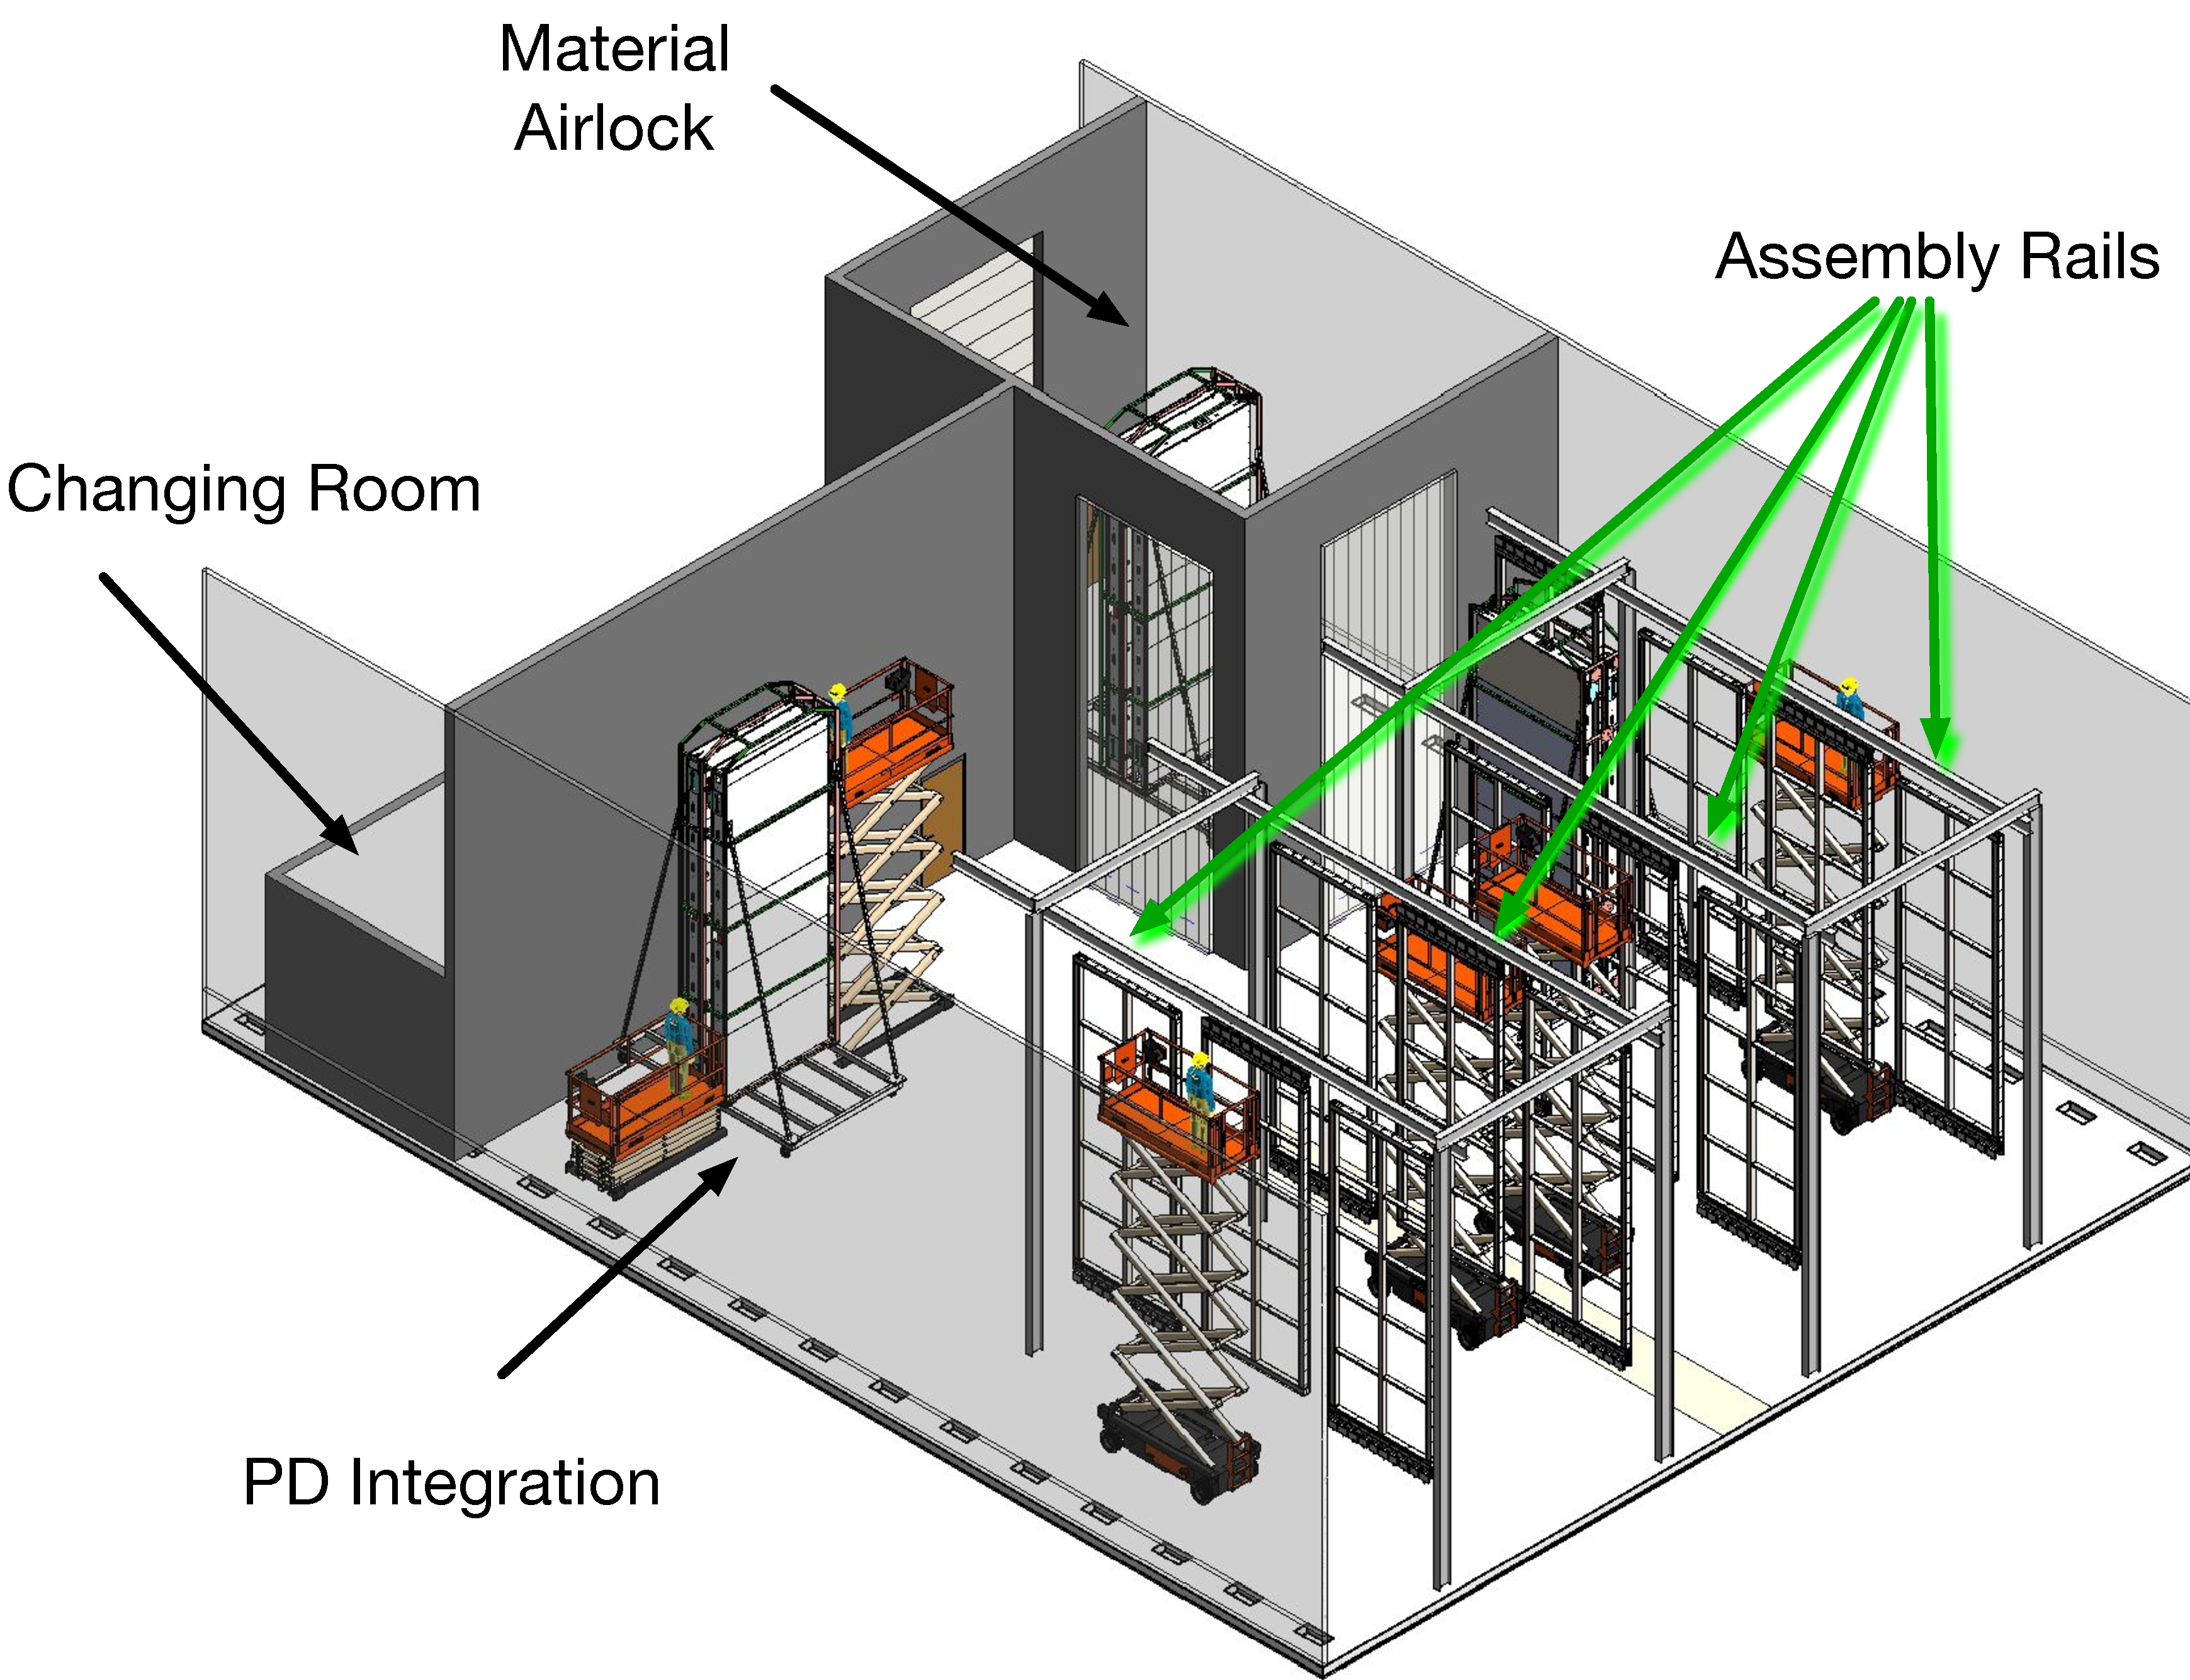
\includegraphics[width=.8\textwidth]{graphics/install-integrate-rail.pdf}
\end{dunefigure}


Given the substantial size and the significant occupancy of the cleanroom, it will require electrical outlets, Wi-Fi, and fire protection. Monitoring for \dword{odh} will be installed as required by the safety analysis of the coldbox cryogenic system.

Equipment in the integration work area adjacent to the materials airlock will consist of a station for integrating the \dwords{pd} into the \dword{apa}, two pairs of rails for preparing the \dword{apa} for assembly, and several scissor lifts for working around the \dword{apa}s. 
In the \dword{pd} integration area an \dword{apa} transport box will be positioned between two fixed lifts that will be raised until the \dword{pd} paddles can easily be inserted into the side of the \dword{apa}. 
Figure \ref{fig:install-integrate-rail} illustrates the rail setup in the integration work area. 
The \dword{apa}s are removed from their transport box and mounted to the rails at the far end of the assembly rails near the \dword{pd} integration area and material airlock. 
They then move along the rails using simple trolleys running on the I-beams. 
The rails are long enough to hold three \dword{apa}s at a time. 
This setup is conceptual and the engineering design of the rail supports has not yet started. 
Cross bracing of the vertical posts will be added during the design stage. 

\begin{dunefigure}[APA cabling tower]{fig:install-assembly-tower}
  {
  Isomtetric view of the \dword{apa} assembly and cabling tower. The steel outer structure is shown in red. The inner scaffolding in gray permits work at different heights.
  The tower is designed to be two \dword{apa}s wide to allow work on two of them side-by-side simultaneously. 
  Both the north and south faces are equipped with assembly rails so that 
   a single tower can support two assembly lines.
  }
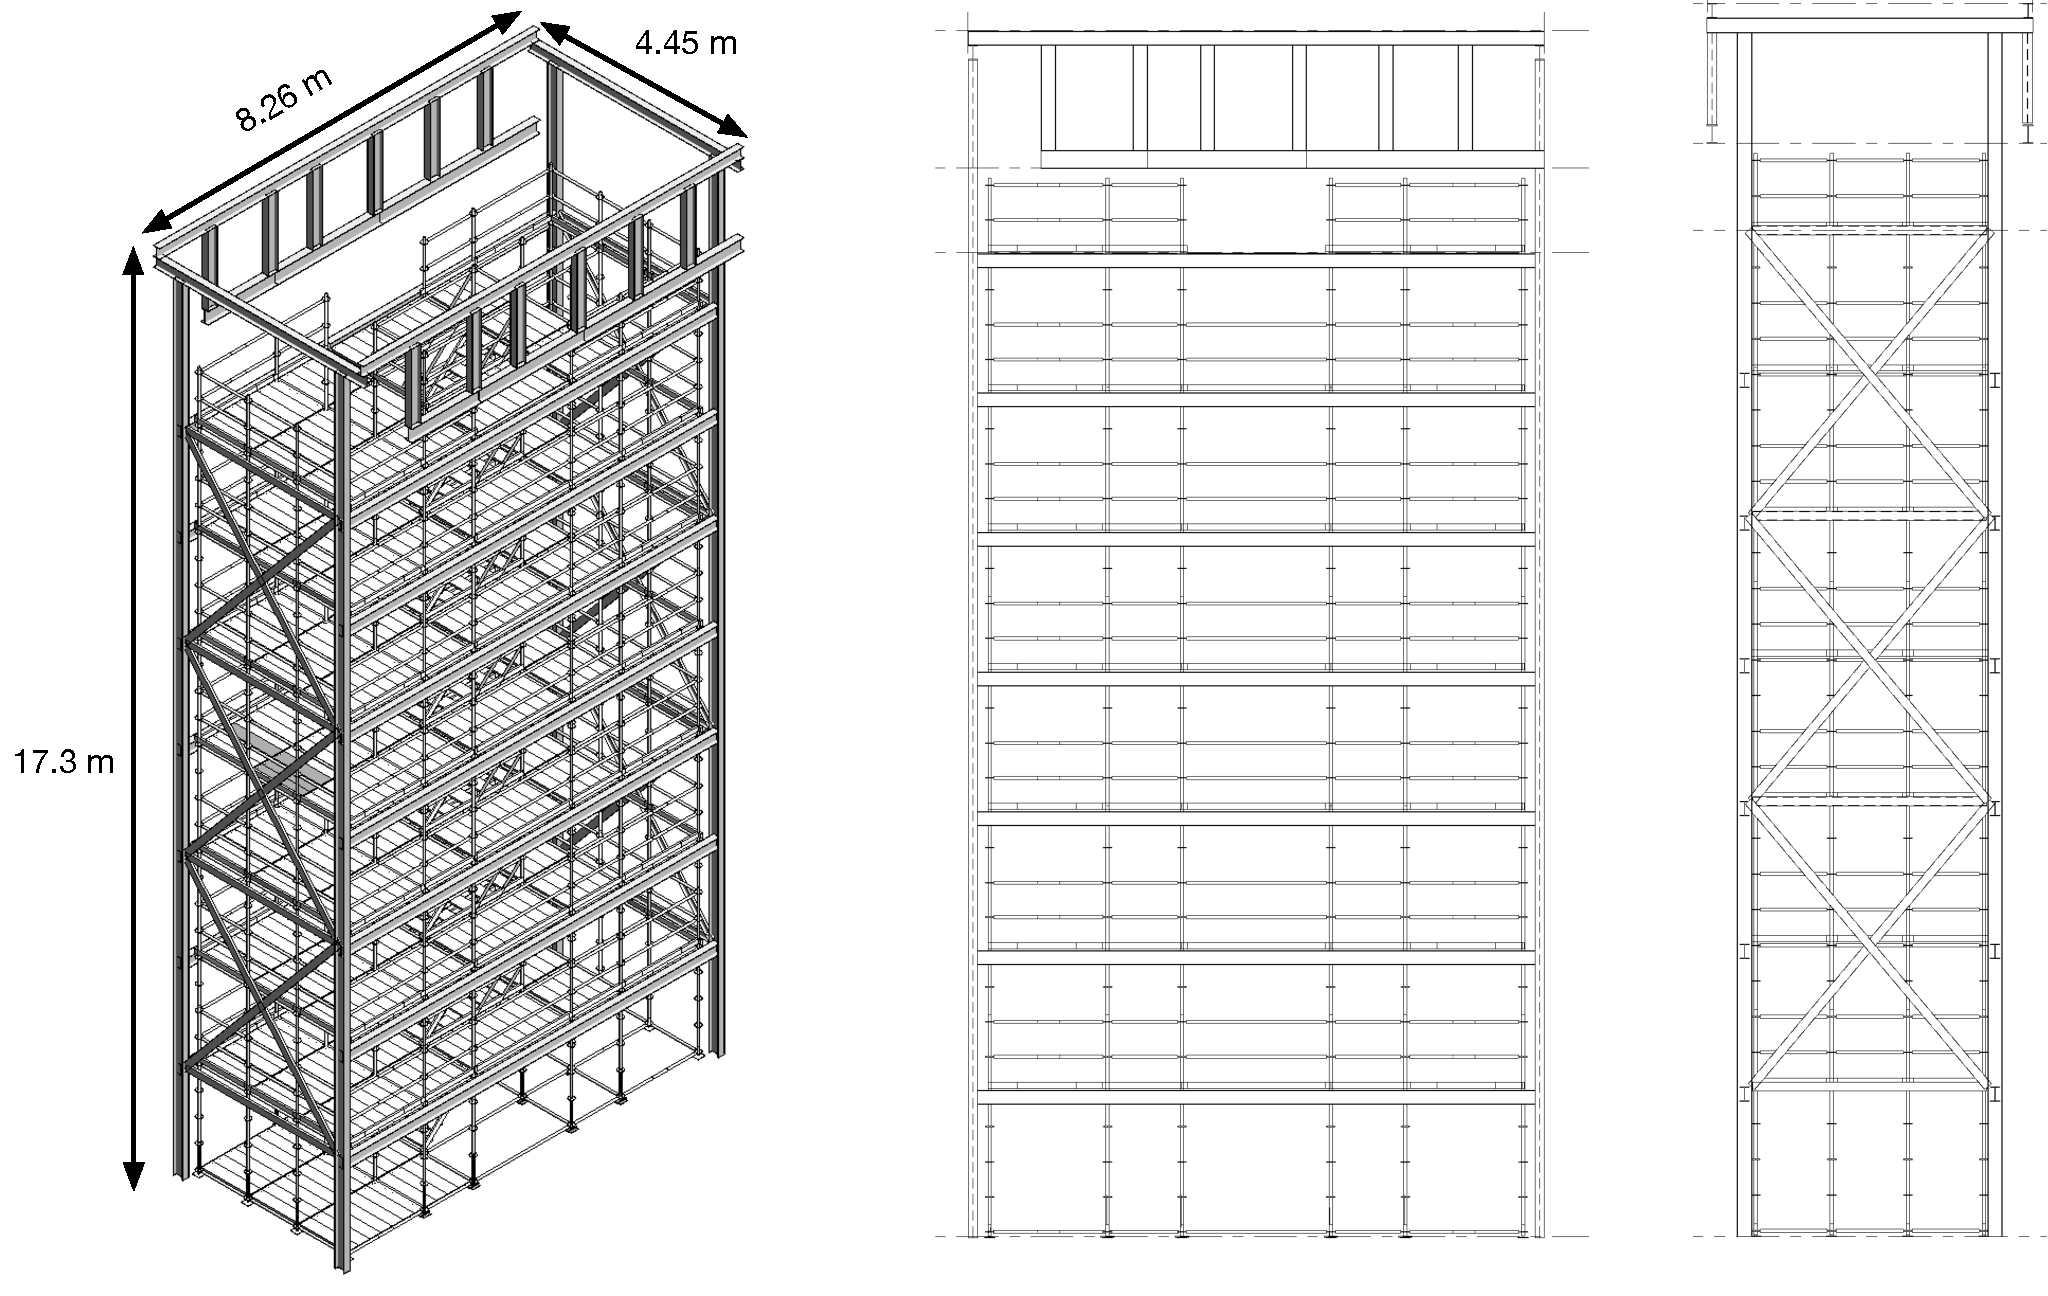
\includegraphics[width=.5\textwidth]{graphics/install-assembly-tower.pdf}
\end{dunefigure}


In the \SI{17}{m} tall  \dword{apa} assembly and cabling area of the cleanroom two large work towers (shown in Figure~\ref{fig:install-assembly-tower}) support the four assembly lines. 
These towers are designed to be wide enough to hold two \dword{apa}s  side-by-side with enough space between them to walk through or work. 
The tower is seven stories tall with work areas at each landing.
Rails at mid-height and at the top of the towers are used to move the \dword{apa}s to the different locations along the tower. 
The towers also provides support for the tooling needed to hold the upper and lower \dword{apa} during assembly and to bring the two modules together so they can be connected. This tooling is called the \dword{apa} assembly fixture and is provided by the \dword{apa} consortium. 

The  tower is conceived as a steel outer frame that supports the \dword{apa}s and the rails. Inside the steel frame is standard scaffolding that allows workers to access the \dword{apa}s at different heights. 
The scaffolding is wide enough for people to work simultaneously on both sides and it accommodates a stairway in the middle that meets \dword{osha} standards. 
North-south beams spanning the width of the cavern will be placed on top of the towers to support the cleanroom roof and the work platforms shown in Figure~\ref{fig:install-workdeck}.
The image shown in Figure~\ref{fig:install-assembly-tower} is a modified model based on a single-wide \dword{apa} tower that has passed all safety reviews and has already been constructed at \dword{ashriver}. 
The double-wide tower will need to be re-engineered to ensure that all the beam dimensions and bracing are appropriate for the larger spans and loads. 
It will then go through the full safety review and an initial prototype 
will be fabricated for use at Ash River. 
The size and the layout of the top level of the tower will be optimized based on input from the Ash River tests. 


\begin{dunefigure}[Cleanroom platforms and material transport system]{fig:install-workdeck}
  {Installation Workdeck, Assembly Towers \&  rails, switchyard, \coldbox{}s and HV assembly area in the installation cleanroom. Plan view. 
  }
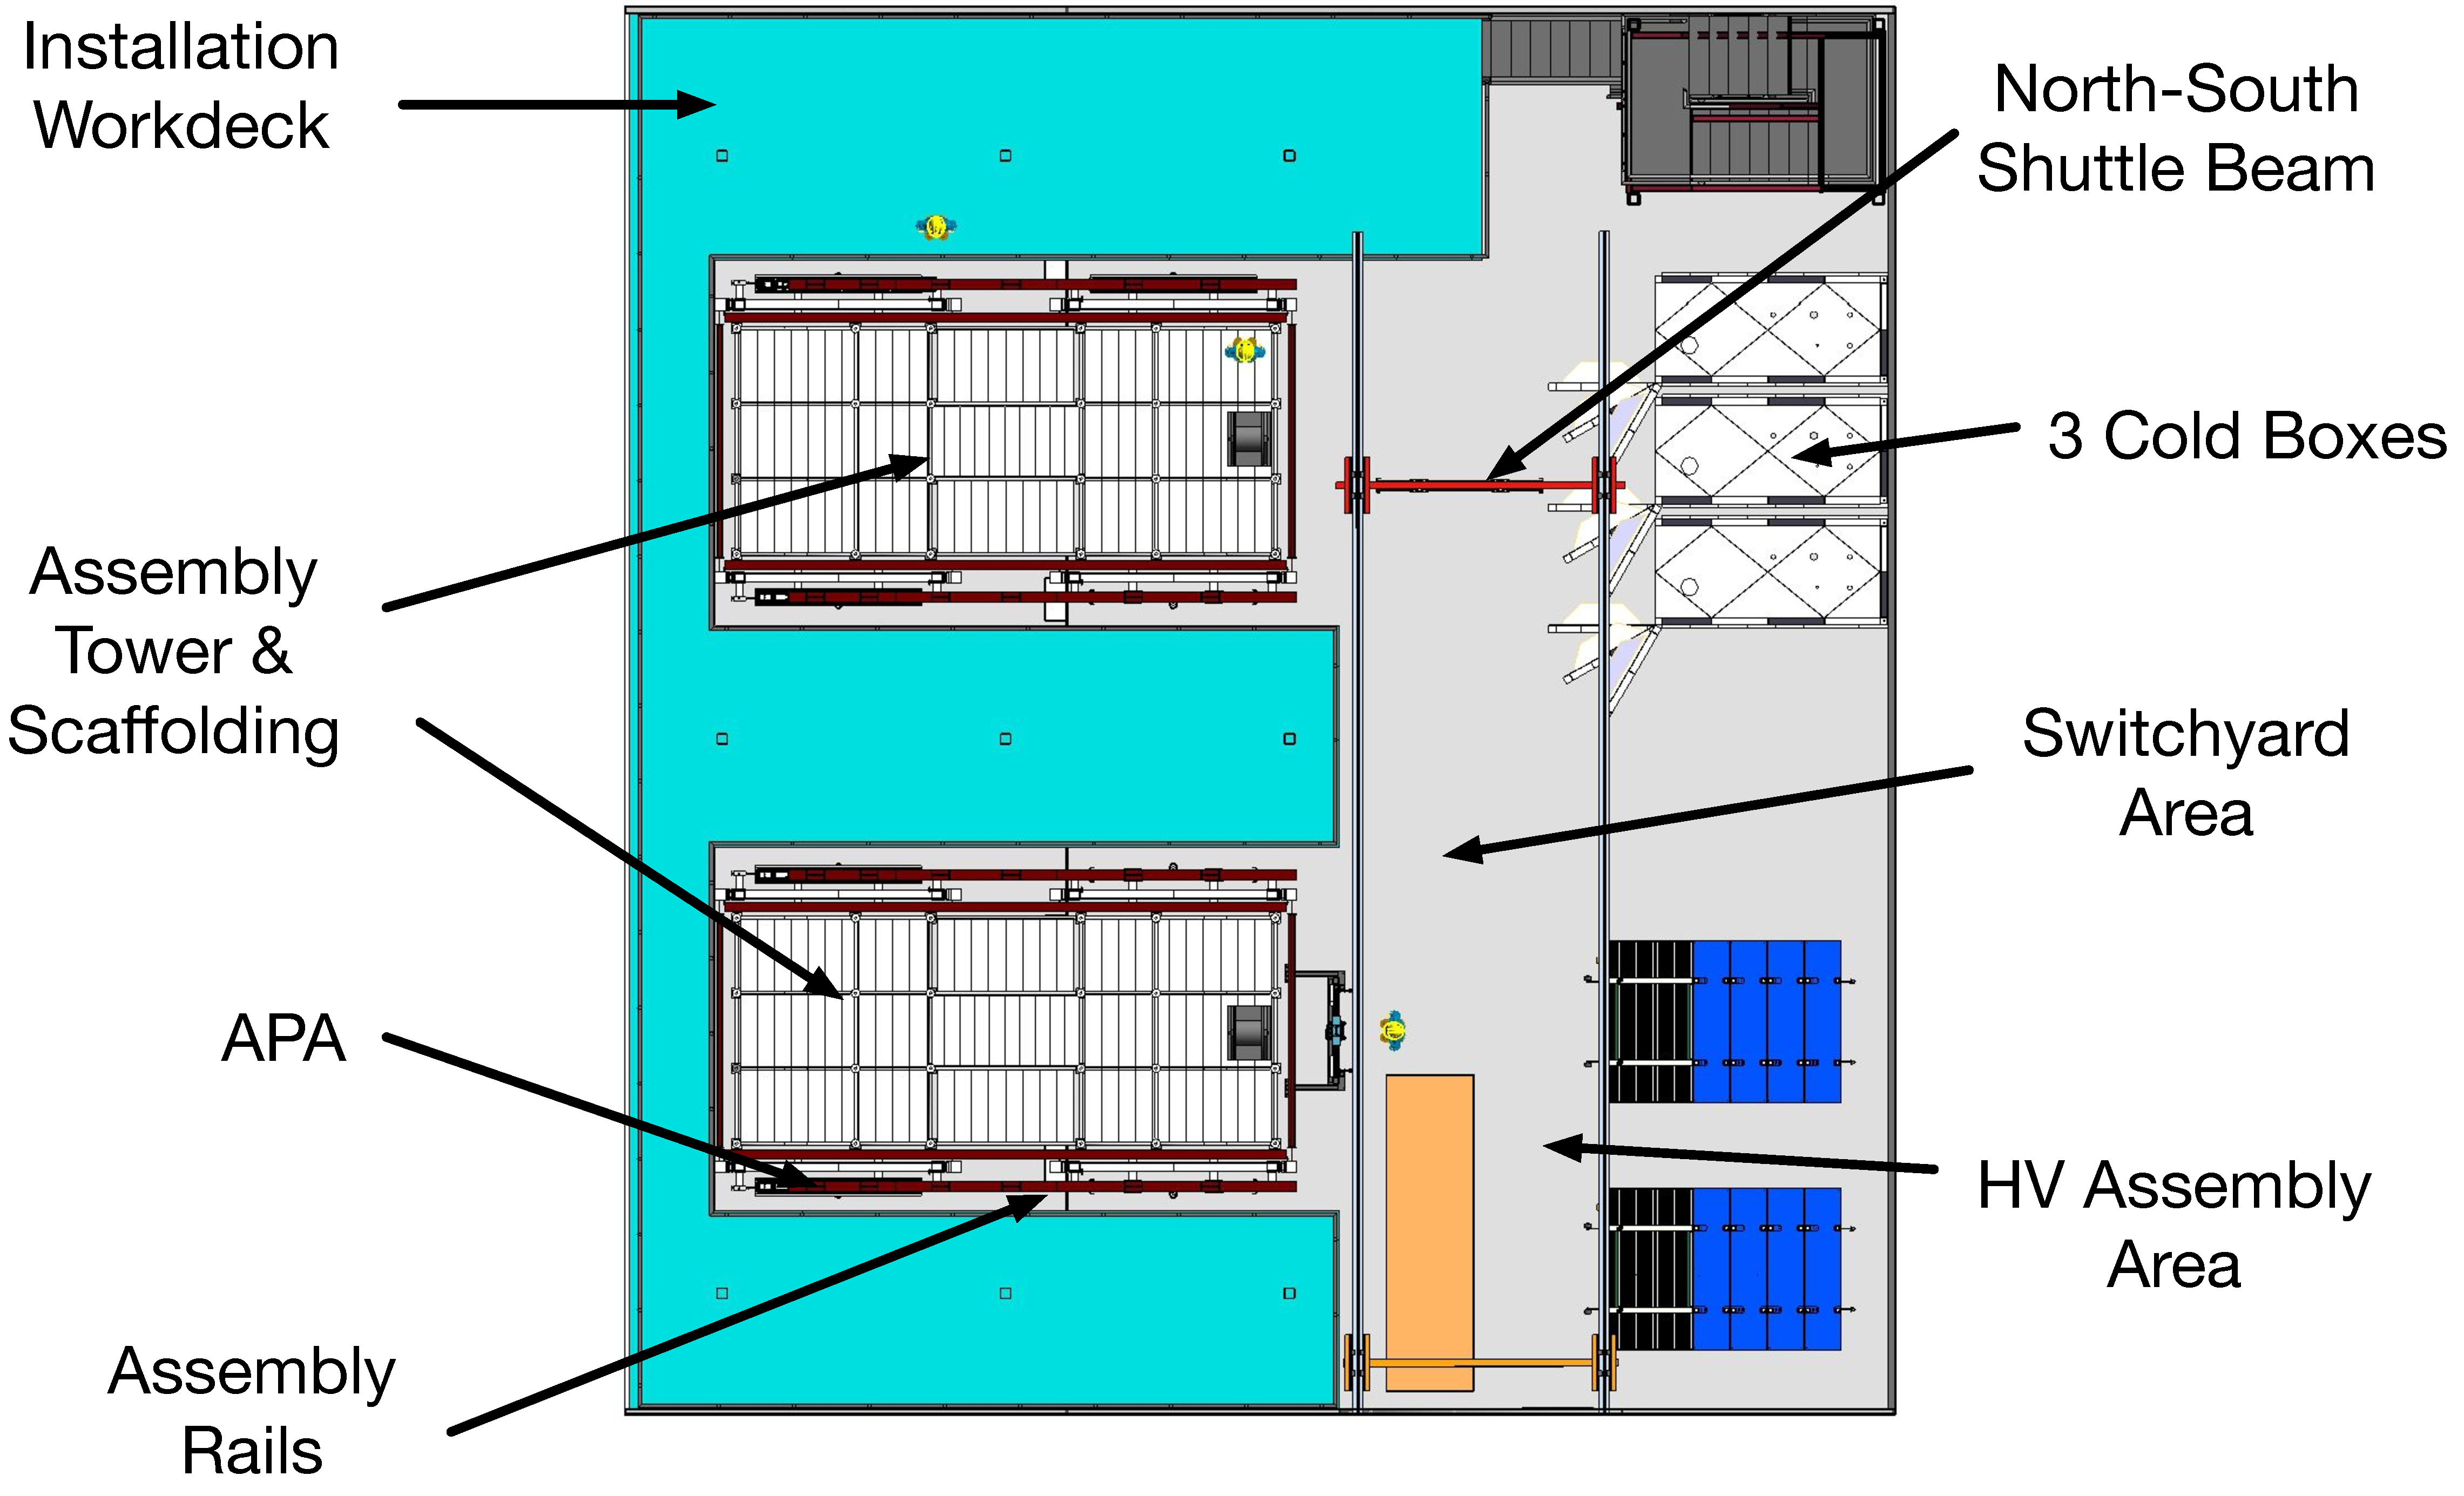
\includegraphics[width=.75\textwidth]{install-workdeck}
\end{dunefigure}

Because the cables can only be inserted through the \dword{apa} frames after the top and bottom \dword{apa}s have been assembled, quite a bit 
of work must be performed at the \SI{14.8}{m} height of the \dword{tco} beam. 

The commercial scaffolding inside the \dword{apa} assembly towers 
provide a solid, safe work platform for working on the side of the \dword{apa} facing the tower. However access to both faces of the \dword{apa} is required to connect the cables to the \dword{femb} and to properly bundle the cable into the cable trays in a way that allows the cables to be installed easily once the assembly is in the cryostat. 
Given the large number of person-hours needed for work at height, all measures will be taken to ensure that this work is safe. 
For this reason a large stable  workdeck will be constructed as shown in Figure~\ref{fig:install-workdeck}.
By running north-south I-beams from the cavern walls across the assembly towers, strong rigid support points are provided. 
Vertical posts down from these beams can then support the fixed workdeck as needed. Access to the workdeck is provided by a walkway along the west end of the platform that connects to both the assembly towers. A second means of egress is also provided by a connection to the permanent stairs. 



Once a top-bottom \dword{apa} pair is assembled it can be moved onto the switchyard under the bridge. 
This switchyard, illustrated schematically in Figure~\ref{fig:install-workdeck}, is essentially a bridge crane running under the north-south bridge in the cavern.  
Several bridge beams (called shuttle beams) driven by electric trolleys  move on the runway beams of the crane.  
A rail at the bottom of the crane mates with the fixed beams  from the assembly lines, the \coldbox{}es, the \dword{tco} beams and the \dword{hv} assembly area.
By aligning the bridge beams with a set of fixed beams supported from the cleanroom roof, the \dword{apa}s and \dword{cpa}s can be transferred from the fixed beams to the bridge crane and moved to different locations in the cleanroom. 
The \SI{12}{m} tall \dword{cpa} panels will be assembled directly under the bridge crane and transferred directly from the assembly fixture to the switchyard crane.

The division of responsibilities between the installation and the consortia deliverables are defined in interface documents, but they are governed by a simple concept. Any part which bolts, pins or connects to a consortia deliverable is the responsibility of the consortia. General infrastructure, hoists, and cranes are the responsibility of the installation team. Thus the installation towers are installation's responsibility while the fixtures that bolt to the towers and to the APAs are the responsibility of the APA consortium. 


%%%%%%%%%%%%%%%%%%%%%%%%%%%%
\subsection{Cryogenics and \Coldbox{}es}
\label{sec:fdsp-tc-infr-cryo}



After an \dword{apa} pair is fully assembled and cabled but before installation in the detector cryostat, it is thermally cycled in a tall narrow test cryostat, called a \coldbox{}, shown in Figure~\ref{fig:install-coldbox}). 
To test \dword{apa}s at a rate necessary to keep up with the installation plan, we will use three identical \coldbox{}es in the cleanroom. 
The \coldbox{}es require a dedicated cryogenics system that uses a fine mist of cold nitrogen to cool down close to \dword{lar} temperature. This system is designed so that no liquid nitrogen will accumulate. 


A \coldbox has external dimensions of 14.0 \si{m} by 3.2 \si{m} by 1.3 \si{m} (H$\times$L$\times$W). With three layers of \SI{100}{mm} thick foam insulation,  
the internal dimensions are 13.4 \si{m} by 2.6 \si{m} by 0.7 \si{m}. A rail section similar to those used elsewhere in the cleanroom will be mounted inside each \coldbox to allow the cleanroom switchyard and trolleys to push an  \dword{apa}  into a \coldbox. The \coldbox{}es will be light-tight when closed to support \dword{pd} testing. A support base under the \coldbox{}es will adjust the height to mate with the cleanroom switchyard.

 
The \coldbox electronics \fdth{}s  will be  similar to what is used on the top of the \dword{dune} cryostat, except that short cables will be run from the \dword{wiec}  to a patch panel inside the \coldbox. This will allow the cable on the \dword{apa} to connect directly to the test readout without having to remove any cabling. The \coldbox  design is nearly the same as the successful \dword{pdsp} \coldbox. The outer shell is similarly constructed of a stainless steel plate with reinforcing ribs welded on. The height is of course doubled, and a hinged door is planned. Unbolting the door and lifting it off the \dword{pdsp} \coldbox required significant effort, and lacking full crane coverage in this case, doors that can be opened and closed using a scissor lift are necessary. The \dword{dune} \coldbox{}es will collectively need about \SI{11}{t} of stainless steel, according to initial estimates. The finished boxes are too big to fit down the Ross Shaft. As the design continues, 
we will investigate whether the boxes can be brought underground partially assembled, or if they must be fully assembled in place.  

The \coldbox{}es and associated cryogenic system are the responsibility of the \dword{jpo} and the design of the \coldbox{}es will be provided by the \dword{cern} team which designed the ProtoDUNE test cryostats. The cryogenic system will be designed by the \dword{lbnf} cryogenic team. 

\begin{dunefigure}[Installation \coldbox]{fig:install-coldbox}
  {\coldbox{}es used to thermally cycle the fully assembled APA pairs. }
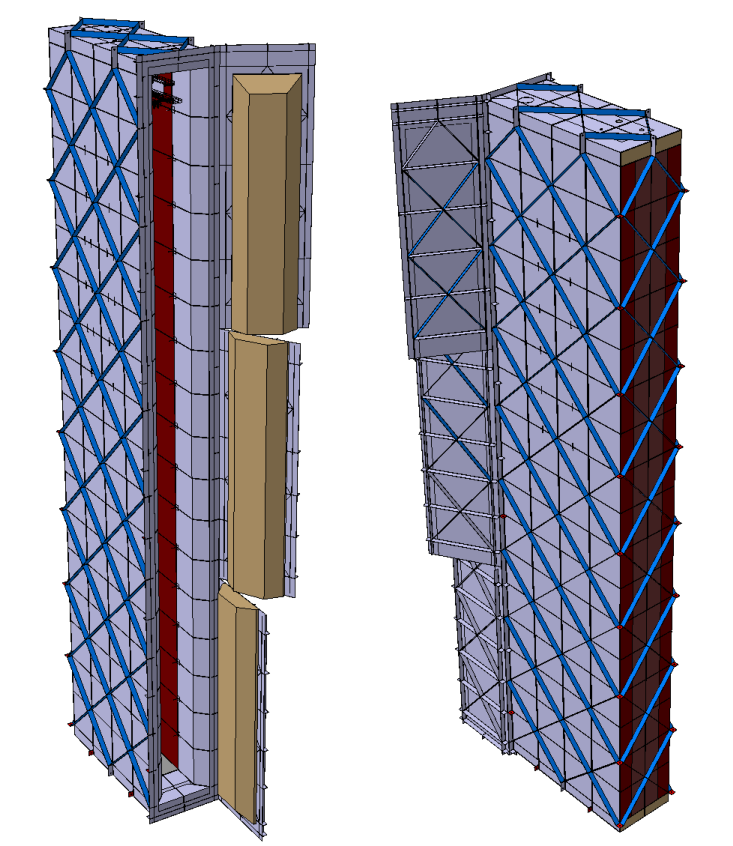
\includegraphics[width=.5\textwidth]{graphics/install-coldbox.pdf}
\end{dunefigure}


%{Cold Boxes Cryogenics}
\label{sec:fdsp-tc-cryocoldbox}


The  \coldbox{}es will be used to test the \dword{apa}s underground prior to installation.  
The cryogenics supporting the \coldbox{}es  must ensure their reliable and safe operation; to that end, the system must
\begin{itemize}
\item support three \coldbox{}es operating in parallel: 
one in \cooldown mode, two either in steady-state or warm-up modes;
\item allow personnel in the cleanroom during all phases of the purge, \cooldown{}, operation, and warm-up modes; 
\item test the detector modules at near \dword{lar} temperature;
\item operate 24 hours a day;
\item allow remote operations; and 
\item be located in the vicinity of the \dword{tco}, as space is available on top of the cryogenics mezzanine on the roof of the cryostat.
\end{itemize}

It must operate in the following modes: 

\begin{itemize}
\item \textbf{purge}: During this mode, air is removed from the system (\coldbox and cryogenics system) and replaced with dry nitrogen. The concentration of moisture is monitored, and when it no longer decreases, the \cooldown can commence.
\item \textbf{\cooldown}: Cold nitrogen is introduced into the system to cool the inside of the \coldbox and the \dword{apa} inside it. 
This should take 24 hours, during which time the temperature decreases from room temperature to about \SI{90}{K}. 
\item \textbf{steady-state operations}: After reaching approximately \SI{90}{K}, 
the detector is turned on and fully tested. 
This takes about 2 shifts.
\item \textbf{warm-up}: After completing the test, the system is
warmed up to room temperature over a period of 24 hours. 
\end{itemize}

\begin{dunetable}
[\Coldbox  cryogenics system parameters] 
{lc}
{tab:table-cryo-coldboxes}
{Table of parameters for the \coldbox cryogenics system}
Parameter & Value 
\\ \toprowrule
Dual \dword{apa} thermal mass &  1,600 kg\\ \colhline
Temperature uniformity & $+60$ K / $-0$ K \\ \colhline
Electronics load & 300 W \\ \colhline
\Coldbox insulation thickness &  0.3 m \\ \colhline
Target \cooldown temperature &  \SI{90}{K} \\ \colhline
Target \cooldown duration &  24 hr \\ \colhline
Target steady-state duration &  24 hr \\ \colhline
Target warm-up duration &  24 hr \\ \colhline
Maximum cooling power  &  \SI{13}{kW}  \\ \colhline 
Maximum liquid nitrogen consumption  &  \SI{300}{l/hr}  \\ 
\end{dunetable}

The evaporation of liquid nitrogen provides the cooling power for the system. Warm nitrogen and a heater provide the heating power. At peak consumption, the expected maximum heat load is \SI{8.5}{kW}. Assuming a 50\% margin on the refrigeration load, the cryogenics system requires \SI{13}{kW} of net cooling power at peak consumption, which equals about \SI{300}{l/hr} of evaporating liquid nitrogen.

Two layouts are currently under consideration: (1) a closed-loop with mechanical refrigeration, in which liquid nitrogen is generated in situ, circulated, and the spent nitrogen recondensed before being put back into the system; and (2) open-loop, in which liquid nitrogen is transported underground by means of portable dewars, circulated, and the spent nitrogen vented away. For the closed-loop, we would need a mechanical refrigeration capable of supplying \SI{13}{kW} of cooling. For the open-loop, it is possible to use a \SI{2000}{l} dewar, which is commercially available and transportable up and down the Ross Shaft inside the cage. To supply the required amount of nitrogen, four trips per day are needed. \fixme{for what period of time? anne}

The current versions of the closed-loop and open-loop systems are presented in Figures~\ref{fig:mechanical-refrigeration} and~\ref{fig:LN2}, respectively. Both options are viable and a decision will be taken on which to adapt after the analysis is complete.

A full \dword{odh} analysis will be performed once the design has progressed to the point where the process flow and pipe dimensions are fixed (These are a necessary input to the analysis).  %Initial assessment is that because 
Since no liquid is accumulated and the room volume is large, our initial assessment is that standard \dword{odh} safety measures will be adequate.

\begin{dunefigure}[\Coldbox cryogenics support system based on mechanical refrigeration ]{fig:mechanical-refrigeration}
  {Layout of the cryogenics supporting the \dword{apa} test facility with mechanical refrigeration (closed-loop).}
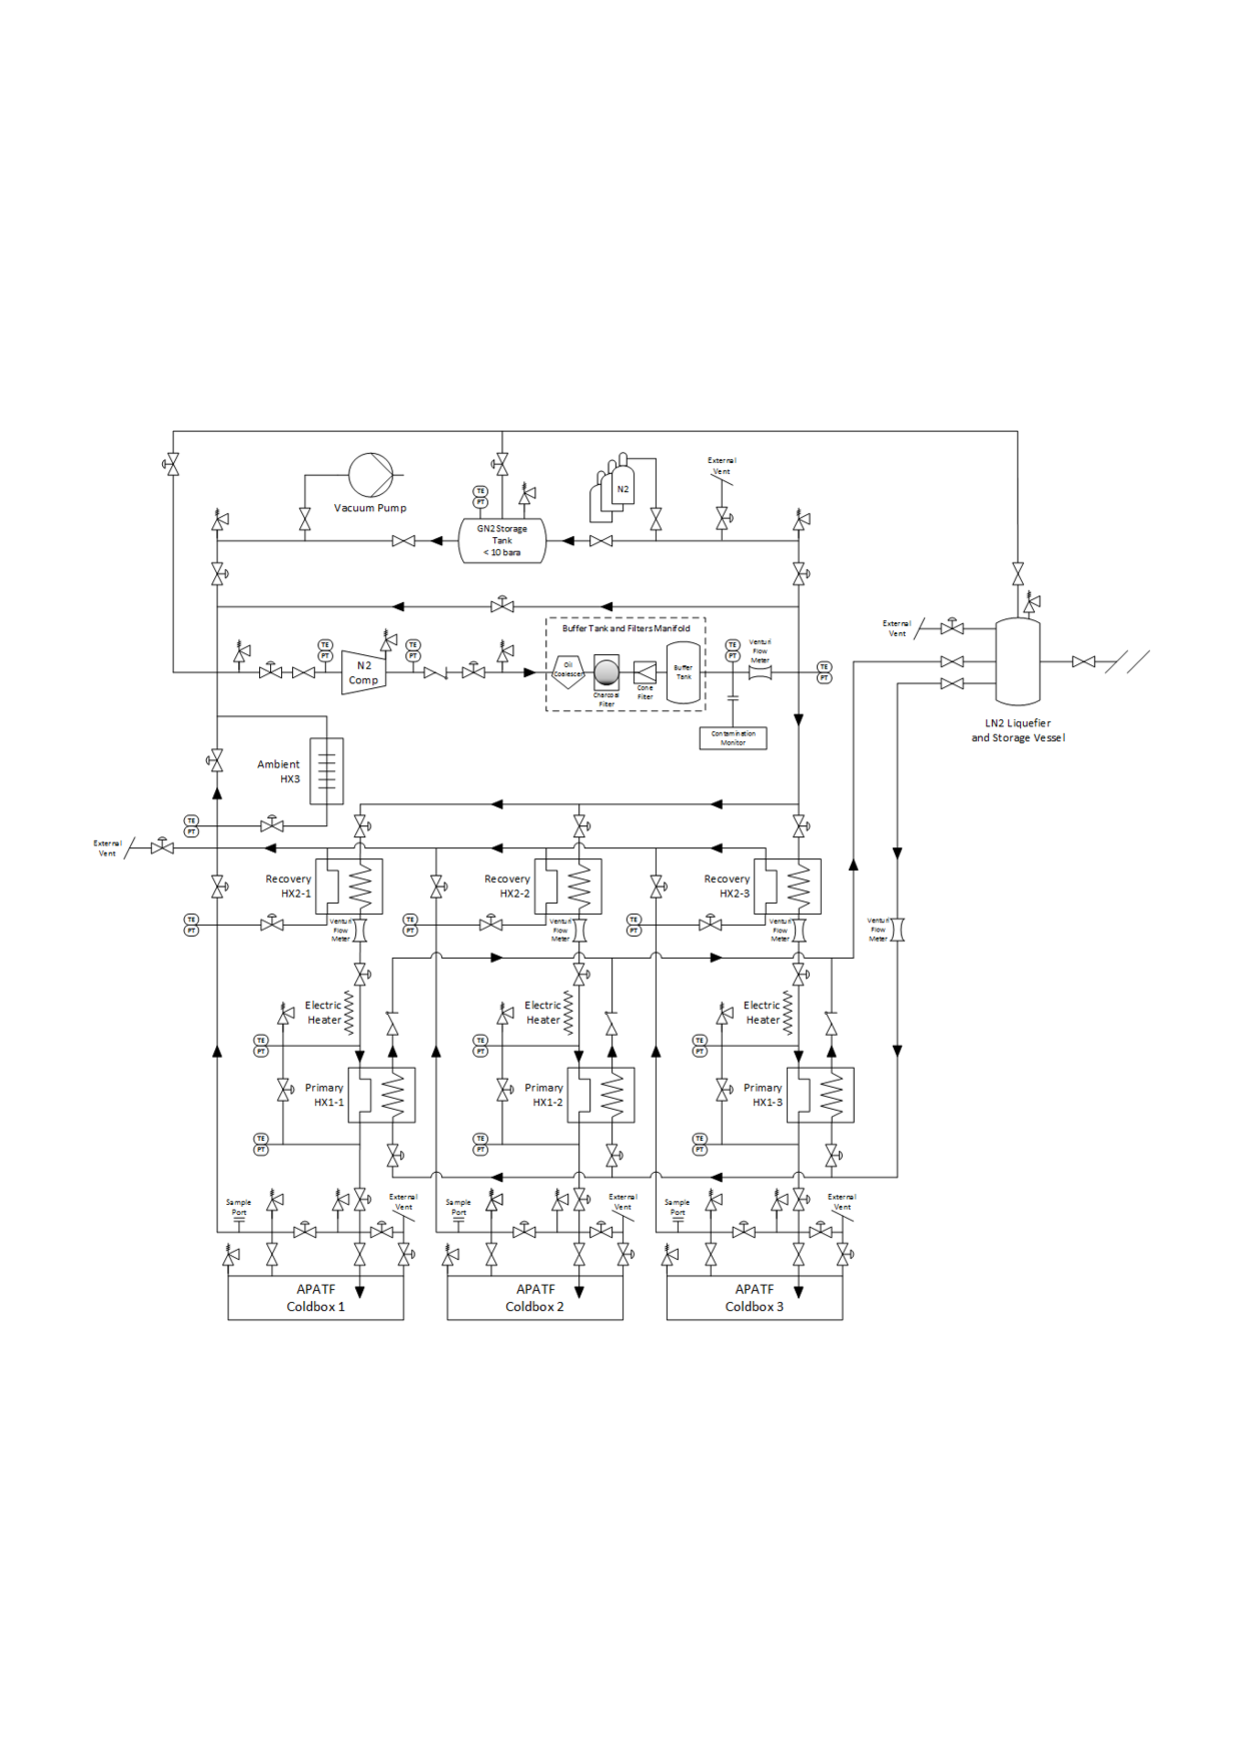
\includegraphics[width=.98\textwidth]{graphics/Cryo-cold-box-mechanical.pdf}
\end{dunefigure}

\begin{dunefigure}[\Coldbox cryogenics support system based on LN2 ]{fig:LN2}
  {Layout of the cryogenics supporting the \dword{apa} test facility with open-loop refrigeration (open-loop).}
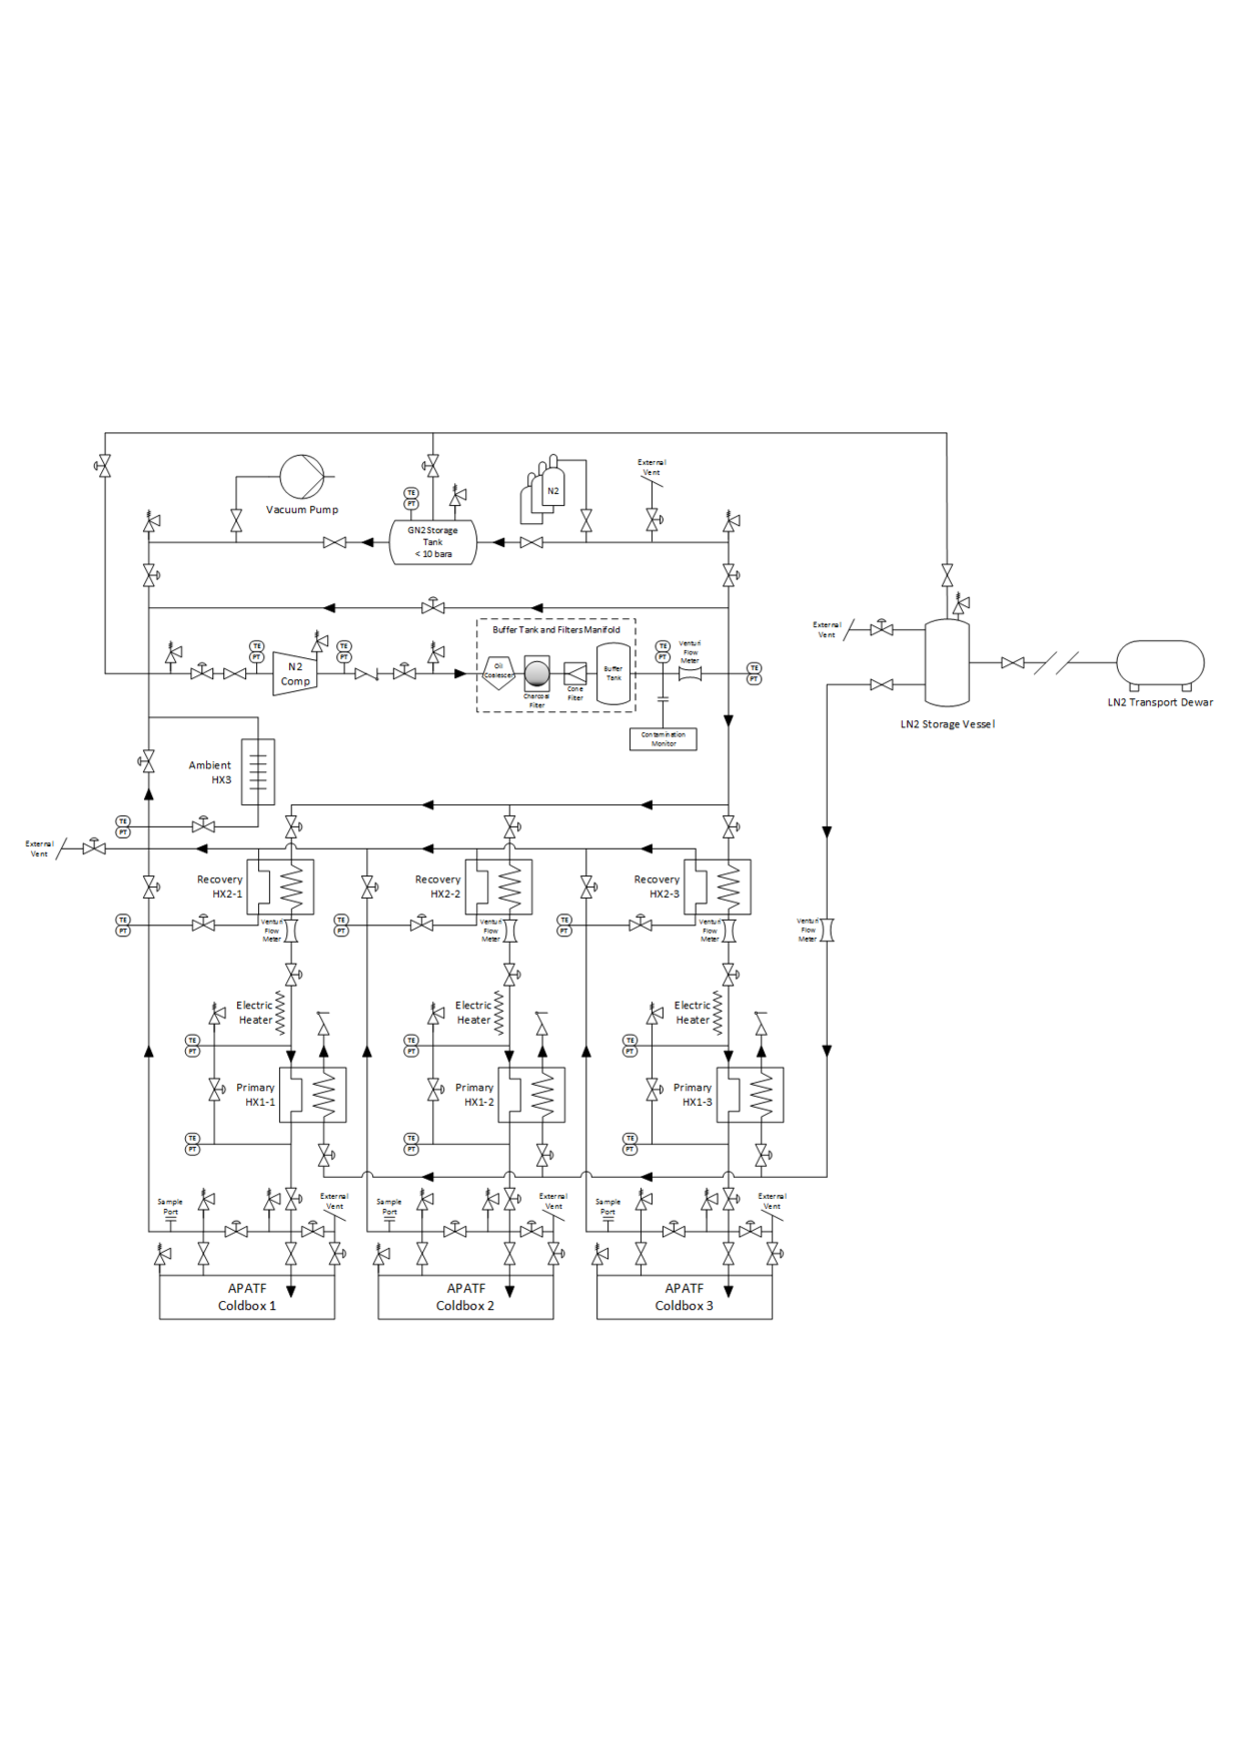
\includegraphics[width=.98\textwidth]{graphics/Cryo-cold-box-LN2.pdf}
\end{dunefigure}



%%%%%%%%%

% clear the figure buffer before starting the next section
\clearpage 

%%%%%%%%%%%%%%%%%%%%%%%%%%%%
\subsection{Prototyping and Testing (QA/QC)}
\label{sec:fdsp-tc-infr-qaqc}


Installing all this new equipment underground during the installation setup phase involves many new techniques  and unique work. While most of the procedures will have been tested during the trial assembly at Ash River, everything must be properly approved. The main \dword{apa} and \dword{cpa} towers will already be structurally approved, but all lifting fixtures, shuttle beams, crane tower connections, and \coldbox connections must undergo load tests. 


The load test program for the lifting fixtures, shuttle beams, crane tower connections, and \coldbox connections will be documented in test procedures in accordance with the \dword{lbnf} \dword{dune} \dword{qa} program.  
These test procedures will (1) list prerequisites for testing, (2) identify fixtures and test equipment, and (3) provide step-by-step instructions, acceptance criteria, and documentation requirements.
They will be in place prior to the start of testing. 
The test results will be documented and approved by the systems engineering team prior to use of the lifting fixtures, shuttle beams, and crane tower connections. The \coldbox connections must undergo load tests. 

The \coldbox{}es and cryogenics system will also be tested, which may require restricting  access to the cleanroom  %may be restricted 
for several days for system checks. 
The \coldbox{}es and the associated cryogenic system test program will be similar to the test program that was instituted for \dword{pdsp}. 
This test program will also be documented in procedures in accordance with the \dword{lbnf} \dword{dune} \dword{qa} program. %The test procedures will include prerequisites prior to testing, identify test equipment, step by step instructions, acceptance criteria and documentation requirements. 
These test procedures will (1) list prerequisites for testing, (2) identify test equipment, and (3) provide step-by-step instructions, acceptance criteria, and documentation requirements.
 The test results will be documented and approved by the systems engineering team prior to use of the \coldbox and cryogenics system.

% clear the figure buffer before starting the next section
%\clearpage